%\documentclass[first,firstsupp,handout,compress,notes,navigation,hyperref,table]{ETHclass}
%\documentclass[first,firstsupp,handout,lastsupp]{ETHclass}
\documentclass[first,firstsupp,lastsupp,last,hyperref,table]{ETHclass}
%\documentclass[first,firstsupp]{ETHclass}
\usepackage{etex}


\usepackage{adjustbox}
\usepackage{amsmath}
\usepackage{amssymb}
\usepackage{animate}
\usepackage{booktabs}
\usepackage{charter}
\usepackage{enumitem}
\usepackage{etoolbox}
\usepackage{ifthen}
\usepackage{longtable}
\usepackage{mathrsfs}
\usepackage{multicol}
\usepackage{pgf}
\usepackage{pgfpages}
\usepackage{pgfplots}
\usepackage{pifont}
\usepackage{ragged2e}
\usepackage{standalone}
\usepackage[caption=false]{subfig}
\usepackage{tabularx}
\usepackage{tikz}
\usepackage{verbatim}
\usepackage{xcolor}
\usepackage{hyperref}

\pgfplotsset{compat=1.7}

\setbeamertemplate{navigation symbols}{}
\usetikzlibrary{arrows,decorations.pathreplacing,positioning,shapes,shadows}

%\usepackage[style=numeric-comp]{biblatex}

%\usepackage{lipsum}

%\usetikzlibrary{fit}
\usetikzlibrary{arrows}
\usetikzlibrary{trees}

% Options for beamer:
%
% 9,10,11,12,13,14,17pt  Fontsizes
%
% compress: navigation bar becomes smaller
% t       : place contents of frames on top (alternative: b,c)
% handout : handoutversion
% notes   : show notes
% notes=onlyslideswithnotes
%
%hyperref={bookmarksopen,bookmarksnumbered} : Needed for menues in
%                                             acrobat. Also need
%                                             pdftex as option or
%                                             compile with
% pdflatex '\PassOptionsToPackage{pdftex,bookmarksopen,bookmarksnumbered}{hyperref} \input{file}'

%\usepackage{beamerseminar}
%\usepackage[accumulated]{beamerseminar}
                                % remove ``accumulated'' option
                                % for original behaviour
%\usepackage{beamerbasenotes}
%\setbeamertemplate{note page}[plain]
%\setbeameroption{notes on second screen}

%\setbeamertemplate{note page}[plain]
%\setbeamertemplate{note page}{\ \\[.3cm]
%\textbf{\color{blue}Notes:}\\%[0.1cm]
%{\footnotesize %\tiny
%\insertnote}}
%\setbeameroption{notes on second screen}


\setbeamertemplate{navigation symbols}{} % suppresses all navigation symbols:
% \setbeamertemplate{navigation symbols}[horizontal] % Organizes the navigation symbols horizontally.
 %\setbeamertemplate{navigation symbols}[vertical] % Organizes the navigation symbols vertically.
% \setbeamertemplate{navigation symbols}[only frame symbol] % Shows only the navigational symbol for navigating frames.

\setlayoutscale{0.5}
\setparametertextfont{\scriptsize}
\setlabelfont{\scriptsize}

% \useoutertheme[subsection=false]{miniframes}
% \usepackage{etoolbox}
% \makeatletter
% \patchcmd{\slideentry}{\advance\beamer@xpos by1\relax}{}{}{}
% \def\beamer@subsectionentry#1#2#3#4#5{\advance\beamer@xpos by1\relax}%
% \makeatother

% \makeatletter
%     \newenvironment{withoutheadline}{
%        \setbeamertemplate{headline}{%
% \vspace{15pt}
% }
%     }{}
% \makeatother

\makeatletter
    \newenvironment{withoutheadline}{
         \setbeamertemplate{headline}{%
\vspace{35pt}
}
        %\def\beamer@entrycode{\vspace*{-1.5\headheight}}
    }{}
\makeatother

\makeatletter
    \newenvironment{tocframe}{
         \setbeamertemplate{headline}{%
\vspace{35pt}
}
         \setbeamertemplate{footline}{%
\leavevmode%
  \hbox{
    \begin{beamercolorbox}[wd=.3\paperwidth,ht=2.5ex,dp=0.75ex,left]{author in head/foot}%
      \qquad\color{white}{\tiny\underline{L. Di Stasio}, J. Varna, Z. Ayadi}%
    \end{beamercolorbox}%

    \begin{beamercolorbox}[wd=.45\paperwidth,ht=2.5ex,dp=0.75ex,center]{title in head/foot}%
      \color{white}{Moscow (RU), April 25-26, 2019}%
    \end{beamercolorbox}%

    \begin{beamercolorbox}[wd=.2\paperwidth,ht=2.5ex,dp=0.75ex,right]{title in head/foot}%
      \color{white}{\insertframenumber\totalframes}%
    \end{beamercolorbox}%
  }
}
        %\def\beamer@entrycode{\vspace*{-1.5\headheight}}
    }{}
\makeatother

\newcommand{\Cross}{$\mathbin{\tikz [x=1.4ex,y=1.4ex,line width=.2ex, red] \draw (0,0) -- (1,1) (0,1) -- (1,0);}$}%

\newcommand{\Checkmark}{$\color{green}\mathbf{\checkmark}$}

\setbeamerfont{subsection in toc}{size=\tiny}

\makeatletter
\patchcmd{\beamer@sectionintoc}
  {\vfill}
  {\vskip1.5\itemsep}
  {}
  {}
\makeatother

\setbeamertemplate{frametitle continuation}{}

\setbeamertemplate{bibliography entry title}{}
\setbeamertemplate{bibliography entry author}{}
\setbeamertemplate{bibliography entry location}{}
\setbeamertemplate{bibliography entry note}{}

\setbeamercolor*{bibliography entry title}{fg=black}
\setbeamercolor*{bibliography entry author}{fg=black}
\setbeamercolor*{bibliography entry location}{fg=black}
\setbeamercolor*{bibliography entry note}{fg=black}
% and kill the abominable icon
%\setbeamertemplate{bibliography item}{\color{forestgreen}$\blacktriangleright$}
\setbeamertemplate{bibliography item}{\insertbiblabel}
%\setbeamertemplate{bibliography item}{\theenumiv}

\newcommand{\highlightred}[1]{%
  \colorbox{red!50}{$\displaystyle#1$}}

\newcommand{\highlightyellow}[1]{%
  \colorbox{yellow!50}{$\displaystyle#1$}}

\newcommand{\highlightgreen}[1]{%
  \colorbox{green!50}{$\displaystyle#1$}}

\AtBeginSection[]{
  \begin{frame}
  \vfill
  \centering
  \begin{beamercolorbox}[sep=8pt,center,shadow=true,rounded=true]{title}
    \usebeamerfont{frametitle}
\includegraphics[width=2ex]{freccia_trasparente_verde_foresta.png}\hspace{.5ex}~{\LARGE \textsc{\bfseries \insertsectionhead}}\par%
  \end{beamercolorbox}
  \vfill
  \end{frame}
}

\hyphenpenalty=5000
\tolerance=1000

\graphicspath{{figures/}}

\newenvironment{system}{\left\lbrace\begin{array}{@{}l@{}}}{\end{array}\right.}

\newenvironment{subsystem}{\left\lgroup\begin{array}{@{}l@{}}}{\end{array}\right.}

\defbeamertemplate*{title page}{customized}[1][]
{
\usebeamerfont{subtitle}
\usebeamercolor[fg]{subtitle}

\vspace{-1.45cm}

{\flushleft
 \usebeamerfont{title}{\inserttitle}\par
}

%\vspace{-.5cm}
\vspace{-.45cm}
{\flushright
\setbeamercolor{author}{bg=white,fg=Red}
\usebeamerfont{author}{\footnotesize \insertauthor} \par}

\vspace{-.35cm}

{\flushright
\usebeamerfont{institute}{\tiny \insertinstitute}\par }

\vspace{.1cm}

{\centering
\usebeamerfont{date}{\scriptsize \insertdate} \par }

\vspace{0.2in}
}


\begin{document}
\setbeamertemplate{caption}{\raggedright\insertcaption\par}

\title{\textsc{growth of interface cracks on consecutive fibers: on the same or on the opposite sides?}}
\author{ \underline{L. Di Stasio}$^{1,2}$, J. Varna$^{1}$, Z. Ayadi$^{2}$}
%\institute{ Science et Ing\'enierie des Mat\'eriaux et M\'etallurgie (SI2M), Institut Jean Lamour, Nancy, France\\Department of Engineering Sciences and Mathematics, Division of Materials Science, Lule\aa\ University of Technology, Lule\aa, Sweden}
\institute{$^{1}$Division of Materials Science, Lule\aa\ University of Technology, Lule\aa, Sweden\\$^{2}$EEIGM \& IJL, Universit\'e de Lorraine, Nancy, France}
\date{12th International Conference on Composite Science and Technology (ICCST/12)\\[-3.5pt]Sorrento (IT), May 8-10, 2019}

\begin{frame}[plain]
    \titlepage

\end{frame}

\begin{tocframe}
\begin{frame}
\frametitle{Outline}
\justifying
\vspace*{-0.5cm}
% \tableofcontents[hidesubsections]
% \begin{multicols}{2}
% \tableofcontents[hidesubsections]
% \end{multicols}
% \begin{columns}[t]
%         \begin{column}{.5\textwidth}
%             \tableofcontents[sections={1-2}]
%         \end{column}
%         \begin{column}{.5\textwidth}
%             \tableofcontents[sections={3-6}]
%         \end{column}
%     \end{columns}
% \end{frame}
\tableofcontents[hidesubsections]
\end{frame}
\end{tocframe}

%\note{}

%\begin{frame}
%\pagediagram
%\end{frame}
%% \note{}

%\section[Transverse Cracking in FRPCs]{Initiation of Transverse Cracking in Fiber Reinforced Polymer Composites (FRPCs): Microscopic Observations \& Modeling}

\section{Micromechanical Modeling of Initiation of Transverse Cracks}

\subsection[Microscopic Observations]{Initiation of Transverse Cracking in FRPCs: Microscopic Observations}

\begin{frame}
\frametitle{\vspace{0.3cm}\small Initiation of Transverse Cracking in FRPCs: Microscopic Observations}
\vspace{-0.5cm}
\centering
\captionsetup[subfigure]{labelfont=footnotesize}
\begin{tikzpicture}

%Tikz axis starts%

\draw[->,black, line width = 5pt] (-4,0) -- (-4,3);
\draw[->,black, line width = 5pt] (-4,0) -- (-4,-3);
\node  at (-4,0) {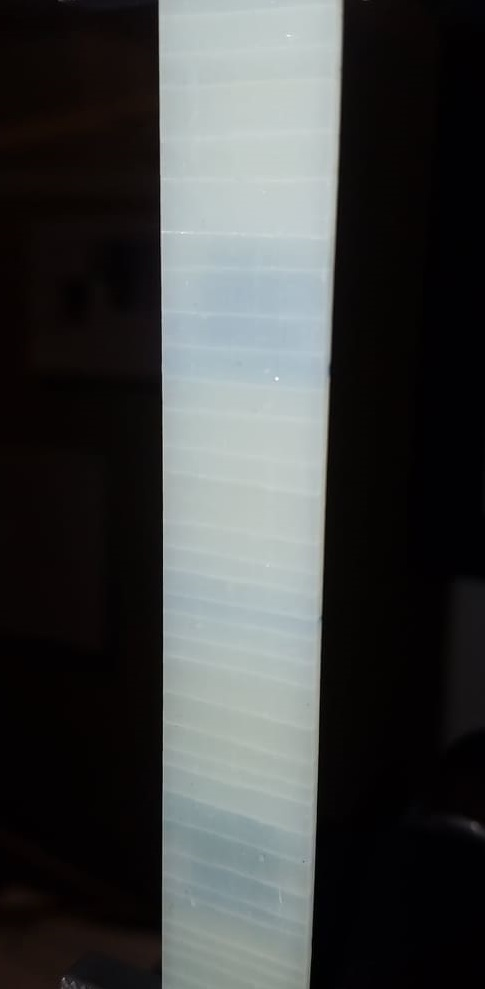
\includegraphics[height=0.6\textheight]{0-90_2_symm}};
\draw[<->,red, line width = 1.25pt] (-4.35,-0.5) -- (-3.65,-0.625);
\node[red, below]  at (-4,-0.65) {\tiny$\mathbf{\sim 15\ mm}$};
\node[above, right]  at (-3.8,3) {\Huge$\mathbf{\varepsilon}$};
\node[below, left]  at (-4.2,-3) {\Huge$\mathbf{\varepsilon}$};

\draw[->,black, line width = 5pt] (-2,0) -- (-2,3);
\draw[->,black, line width = 5pt] (-2,0) -- (-2,-3);
\node  at (-2,0) {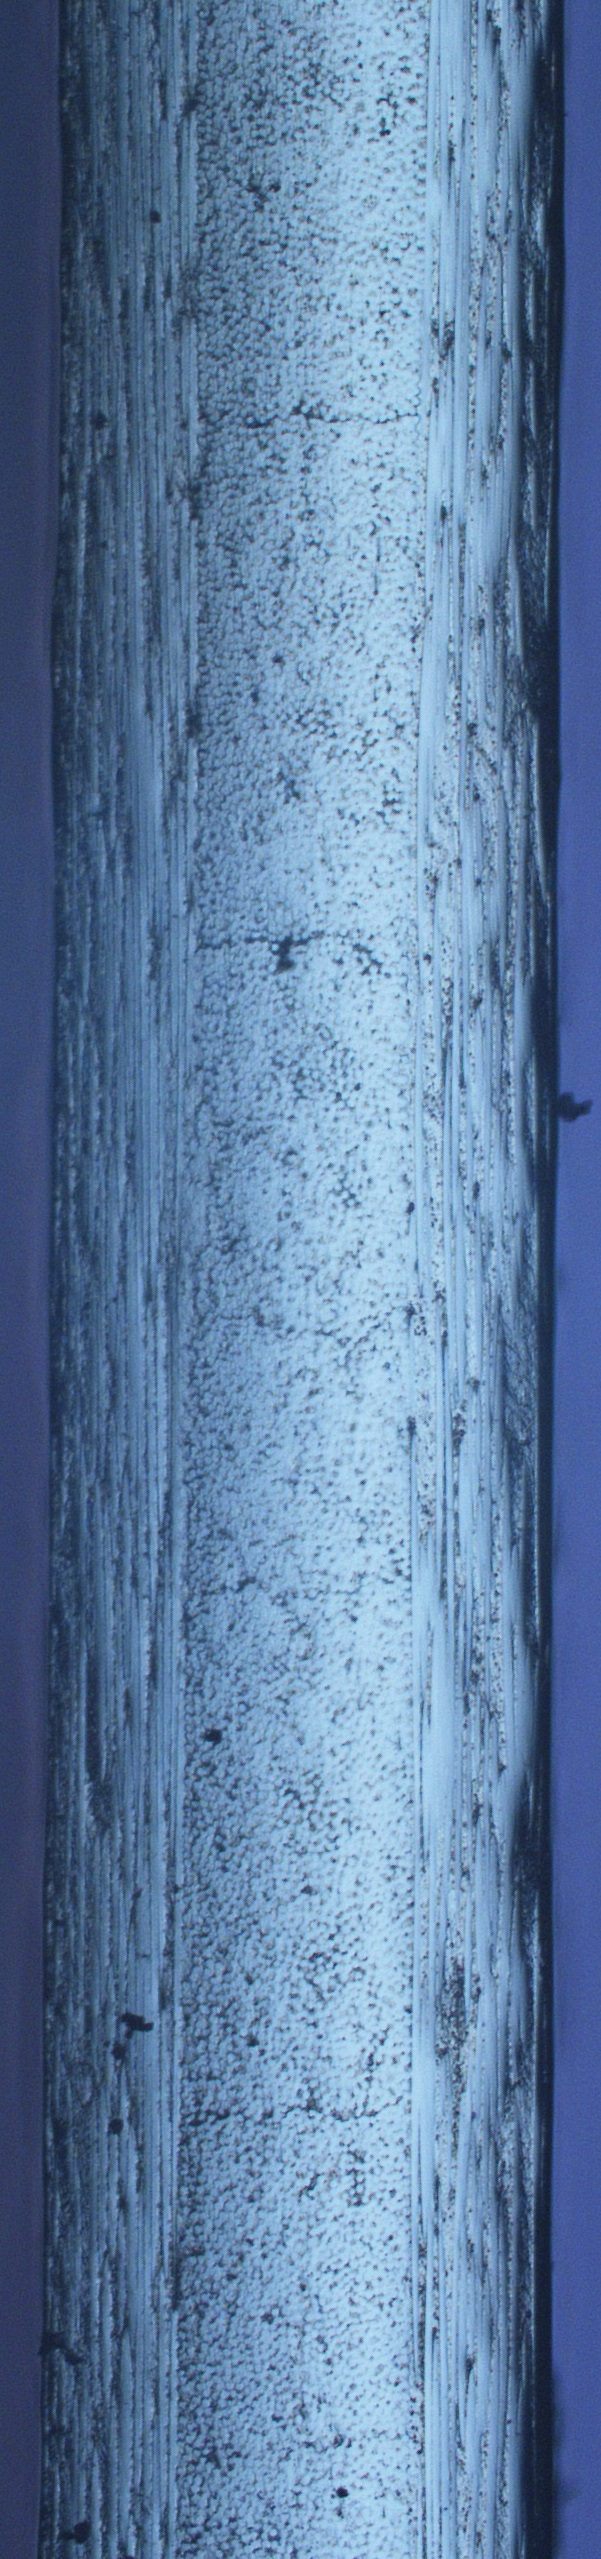
\includegraphics[height=0.6\textheight]{0-90_symm_edge}};
\draw[<->,red, line width = 1.25pt] (-2.46,-0.6) -- (-1.55,-0.6);
\node[red, below]  at (-2,-0.6) {\tiny$\mathbf{\sim 2\ mm}$};
\node[above, right]  at (-1.8,3) {\Huge$\mathbf{\varepsilon}$};
\node[below, left]  at (-2.2,-3) {\Huge$\mathbf{\varepsilon}$};

\draw[->,black, line width = 5pt] (1,0) -- (1,3);
\draw[->,black, line width = 5pt] (1,0) -- (1,-3);
\node  at (1,0) {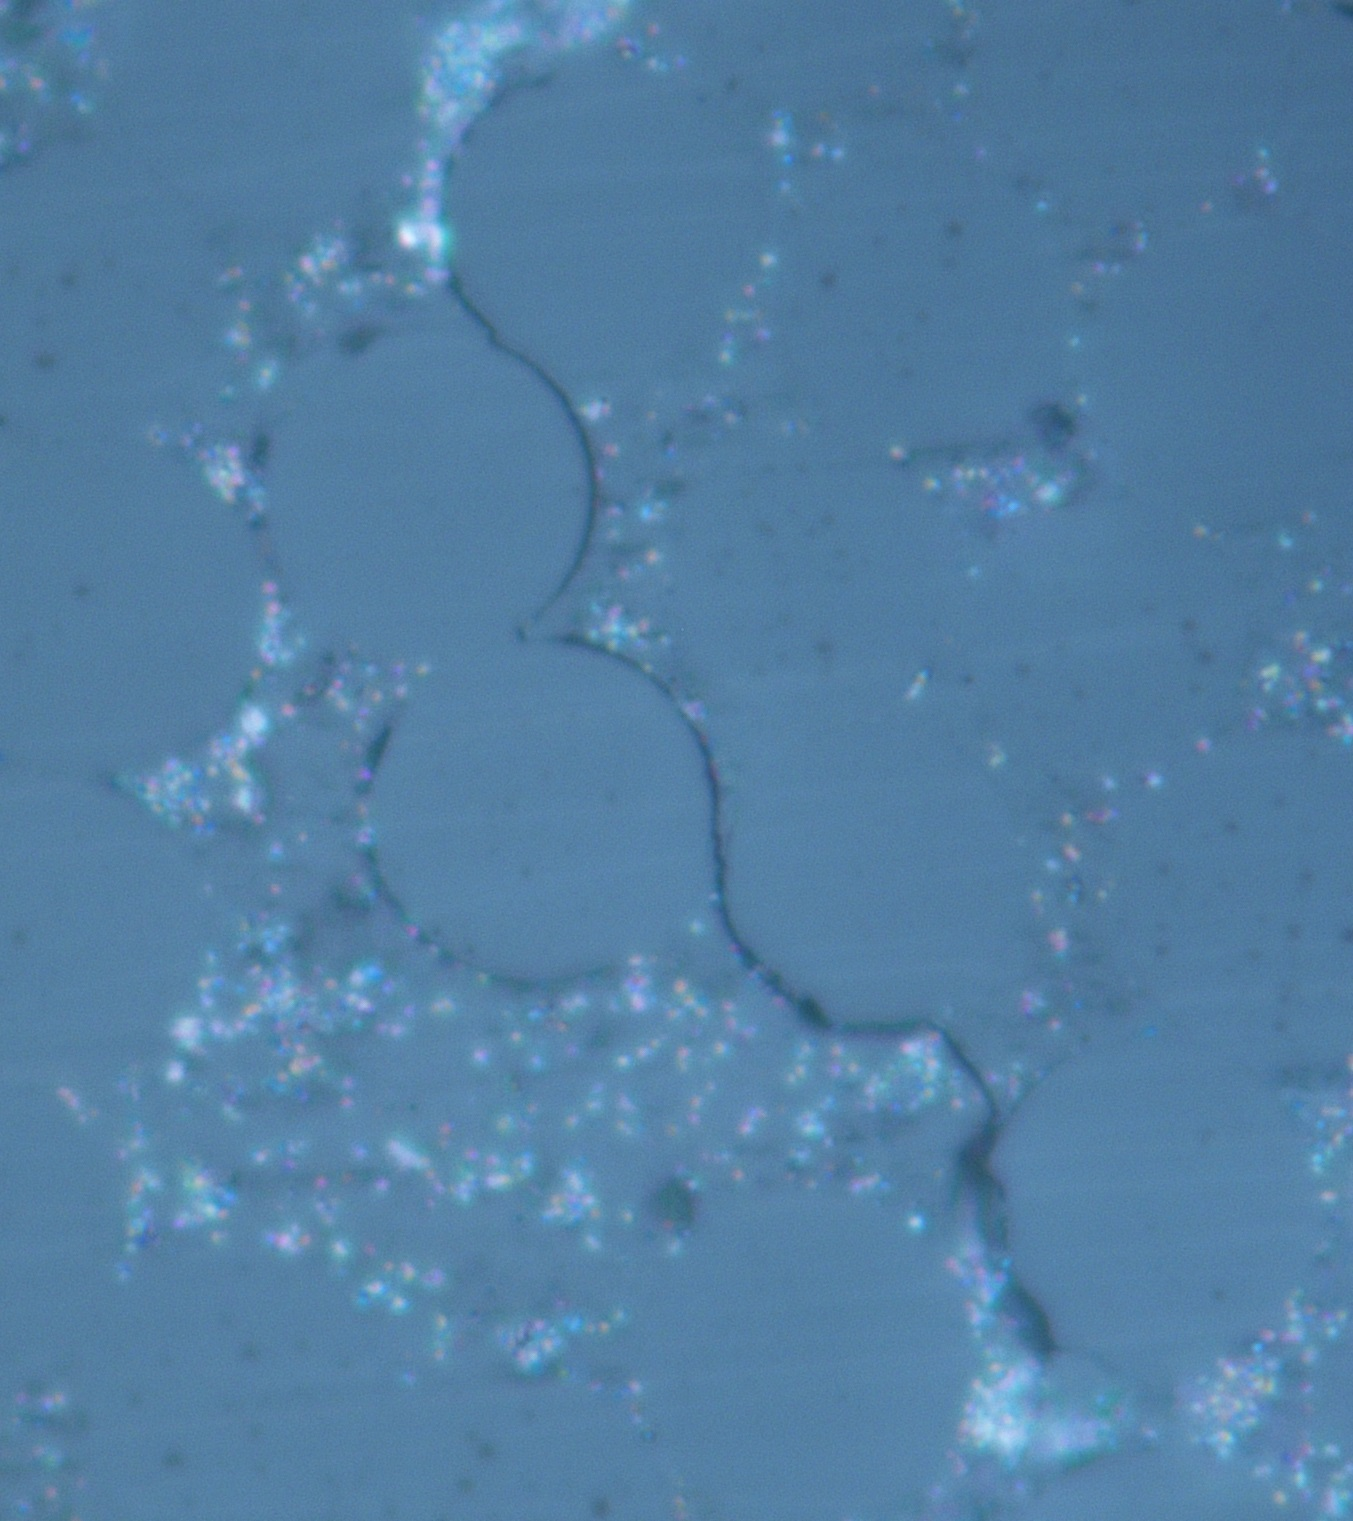
\includegraphics[height=0.6\textheight]{0-90_symm_debondetail}};
\draw[<->,red, line width = 1.25pt] (0.075,-0.15) -- (1.1,-0.15);
\node[red, below]  at (0.55,-0.16) {\tiny$\mathbf{\sim 8\ \mu m}$};
\node[above, right]  at (1.2,3) {\Huge$\mathbf{\varepsilon}$};
\node[below, left]  at (0.8,-3) {\Huge$\mathbf{\varepsilon}$};

\node[anchor=south west]  at (3.25,1.55) {\scriptsize\textbf{Left:}};
\node[anchor=west]  at (3.25,1.5) {\scriptsize front view of $\left[0,90_{2}\right]_{S}$,};
\node[anchor=north west]  at (3.25,1.5) {\scriptsize visual inspection.};

\node[anchor=south west]  at (3.25,0.05) {\scriptsize\textbf{Center:}};
\node[anchor=west]  at (3.25,0) {\scriptsize  edge view of $\left[0,90\right]_{S}$,};
\node[anchor=north west]  at (3.25,0) {\scriptsize optical microscope.};

\node[anchor=south west]  at (3.25,-1.45) {\scriptsize\textbf{Right:}};
\node[anchor=west]  at (3.25,-1.5) {\scriptsize edge view of $\left[0,90\right]_{S}$,};
\node[anchor=north west]  at (3.25,-1.5) {\scriptsize optical microscope.};

%Tikz axis ends%

\end{tikzpicture}
\end{frame}

\subsection[Micromechanics of Initiation]{Initiation of Transverse Cracking in FRPCs: Micromechanics}

\begin{frame}
\frametitle{\vspace{0.2cm}\small Initiation of Transverse Cracking in FRPCs: Micromechanics}
\vspace{-0.75cm}
\centering
\begin{alertblock}{\centering\scriptsize\bf Stage 1: isolated debonds}
\begin{figure}
\centering
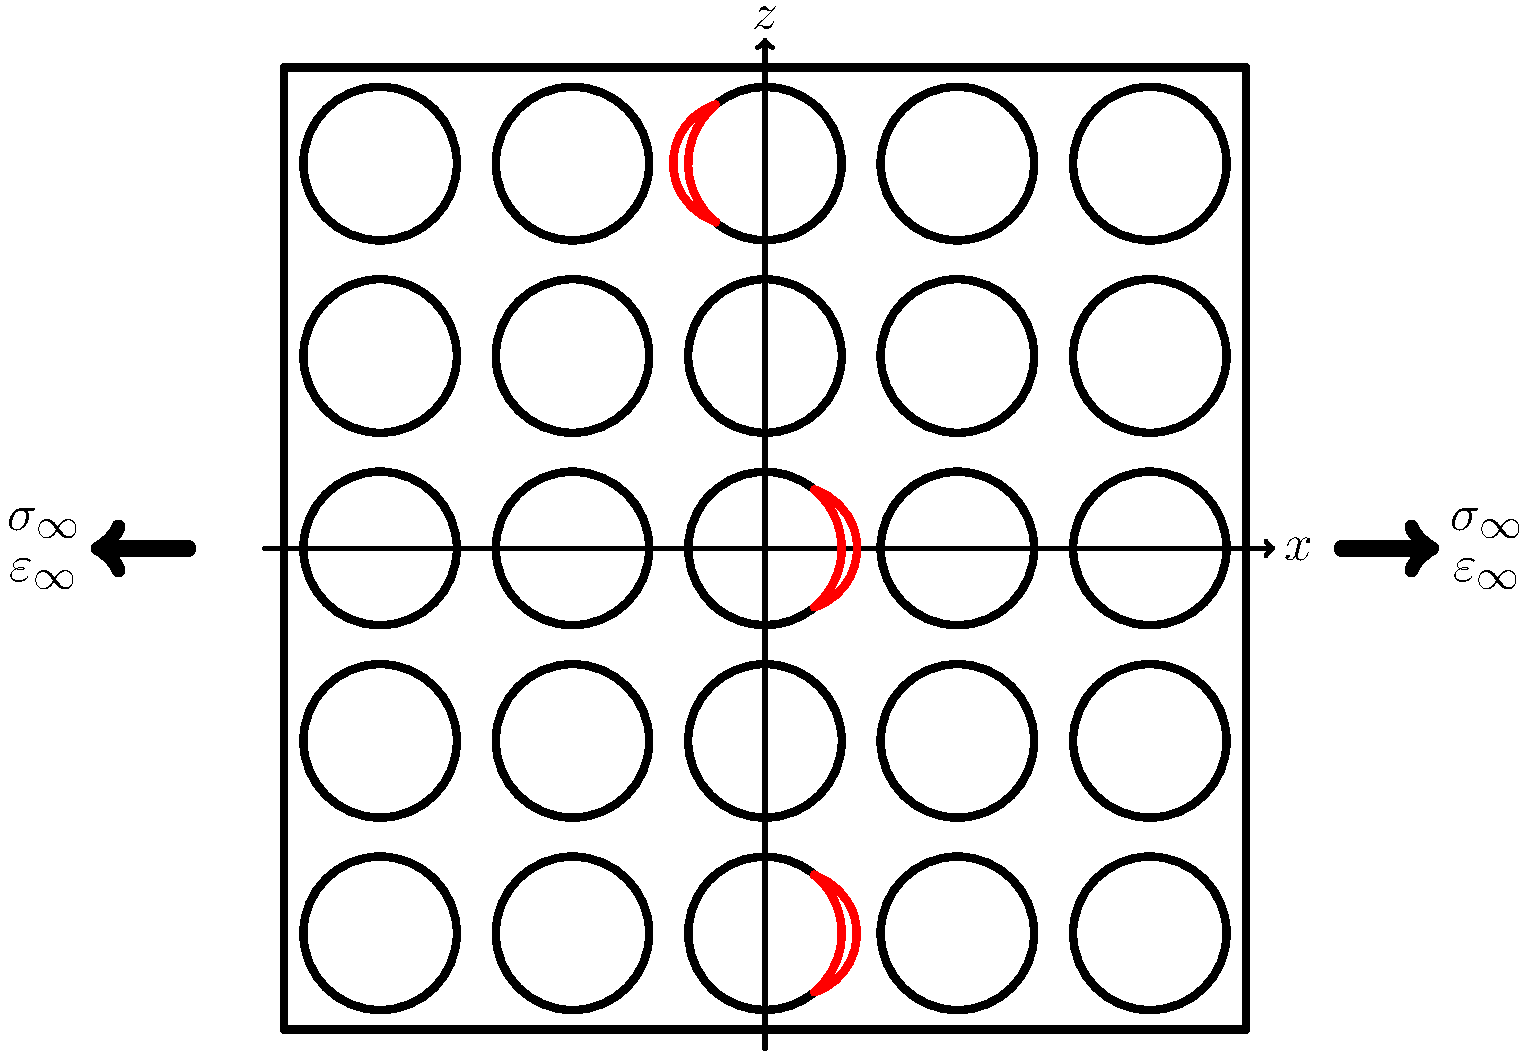
\includegraphics[width=0.6\textwidth]{stage1-isolateddebonds.pdf}
\end{figure}
\end{alertblock}
\vspace{-0.5cm}
%{\tiny J. E. Bailey, P. T. Curtis, A. Parvizi, 1979. {\em\tiny On the transverse cracking and longitudinal splitting behaviour of glass and carbon fibre reinforced epoxy cross ply laminates and the effect of Poisson and thermally generated strain}. {\it\tiny P. Roy. Soc. A-Math. Phy.} {\bf\tiny 366} (1727) pp. 599--623.}
%{\tiny Bailey, J. E., Parvizi, A.; 1981. {\em\tiny On fibre debonding effects and the mechanism of transverse-ply failure in cross-ply laminates of glass fibre/thermoset composites}. {\it\tiny J. Mater. Sci.} {\bf\tiny 16} (3) pp. 649--659.}
{\tiny Zhang, H., Ericson, M. L., Varna, J., Berglund, L.A.; 1997. {\em\tiny Transverse single-fibre test for interfacial debonding in composites: 1. Experimental observations}. {\it\tiny Compos. Part A-Appl. S.} {\bf\tiny 28} (4) pp. 309--315.}
\end{frame}

\begin{frame}
\frametitle{\vspace{0.2cm}\small Initiation of Transverse Cracking in FRPCs: Micromechanics}
\vspace{-0.75cm}
\centering
\begin{alertblock}{\centering\scriptsize\bf Stage 2: consecutive debonds}
\begin{figure}
\centering
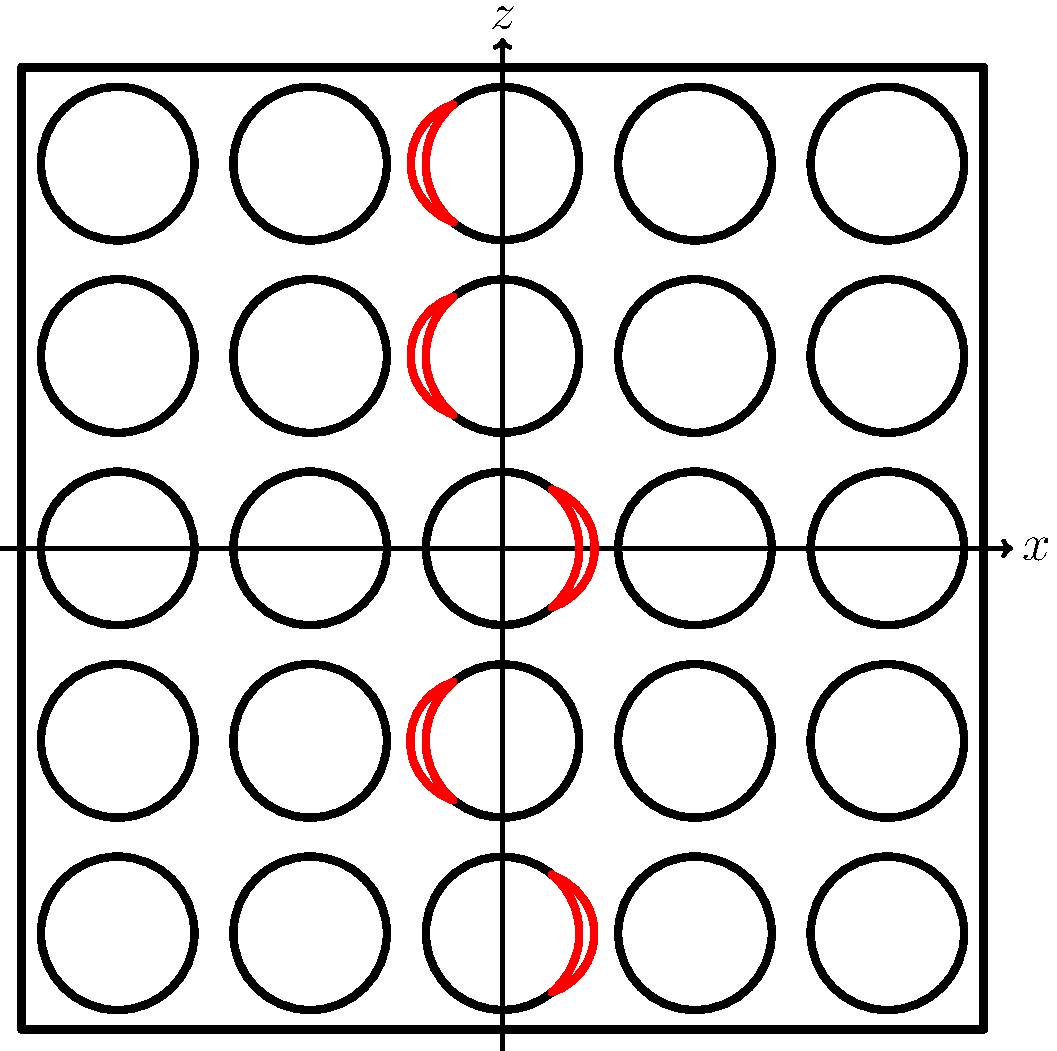
\includegraphics[width=0.6\textwidth]{stage2-critdebonds.pdf}
\end{figure}
\end{alertblock}
\vspace{-0.5cm}
%{\tiny J. E. Bailey, P. T. Curtis, A. Parvizi, 1979. {\em\tiny On the transverse cracking and longitudinal splitting behaviour of glass and carbon fibre reinforced epoxy cross ply laminates and the effect of Poisson and thermally generated strain}. {\it\tiny P. Roy. Soc. A-Math. Phy.} {\bf\tiny 366} (1727) pp. 599--623.}
%{\tiny Bailey, J. E., Parvizi, A.; 1981. {\em\tiny On fibre debonding effects and the mechanism of transverse-ply failure in cross-ply laminates of glass fibre/thermoset composites}. {\it\tiny J. Mater. Sci.} {\bf\tiny 16} (3) pp. 649--659.}
{\tiny Zhang, H., Ericson, M. L., Varna, J., Berglund, L.A.; 1997. {\em\tiny Transverse single-fibre test for interfacial debonding in composites: 1. Experimental observations}. {\it\tiny Compos. Part A-Appl. S.} {\bf\tiny 28} (4) pp. 309--315.}
\end{frame}

\begin{frame}
\frametitle{\vspace{0.2cm}\small Initiation of Transverse Cracking in FRPCs: Micromechanics}
\vspace{-0.75cm}
\centering
\begin{alertblock}{\centering\scriptsize\bf Stage 3: kinking}
\begin{figure}
\centering
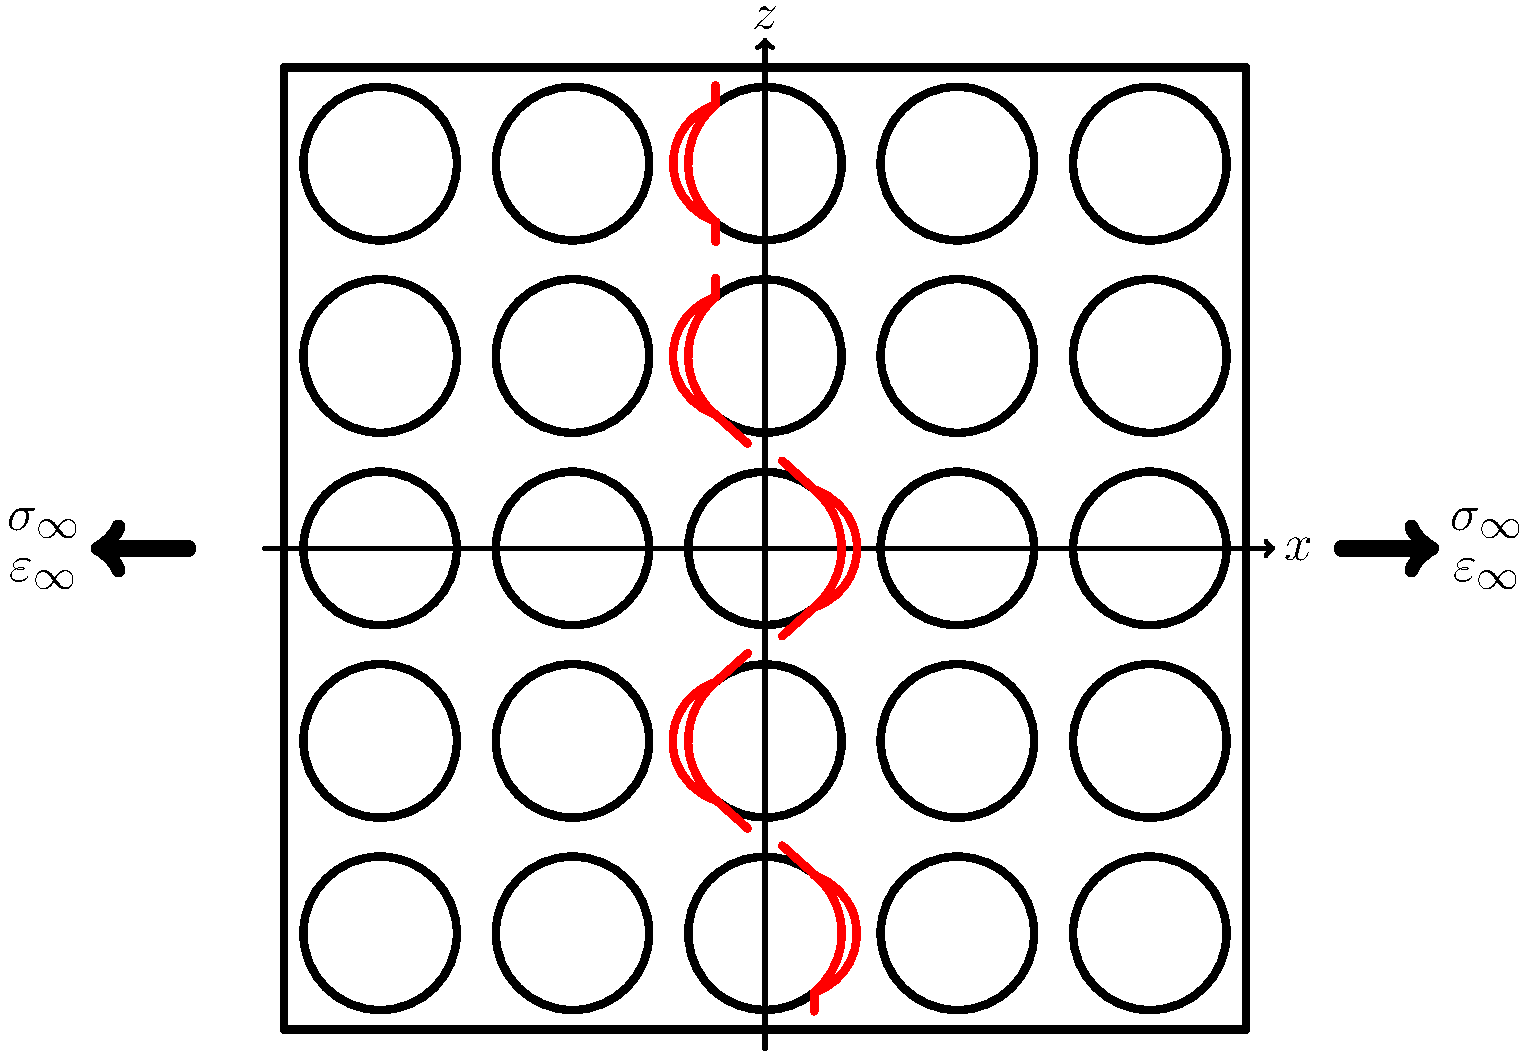
\includegraphics[width=0.6\textwidth]{stage3-kinking.pdf}
\end{figure}
\end{alertblock}
\vspace{-0.5cm}
%{\tiny J. E. Bailey, P. T. Curtis, A. Parvizi, 1979. {\em\tiny On the transverse cracking and longitudinal splitting behaviour of glass and carbon fibre reinforced epoxy cross ply laminates and the effect of Poisson and thermally generated strain}. {\it\tiny P. Roy. Soc. A-Math. Phy.} {\bf\tiny 366} (1727) pp. 599--623.}
%{\tiny Bailey, J. E., Parvizi, A.; 1981. {\em\tiny On fibre debonding effects and the mechanism of transverse-ply failure in cross-ply laminates of glass fibre/thermoset composites}. {\it\tiny J. Mater. Sci.} {\bf\tiny 16} (3) pp. 649--659.}
{\tiny Zhang, H., Ericson, M. L., Varna, J., Berglund, L.A.; 1997. {\em\tiny Transverse single-fibre test for interfacial debonding in composites: 1. Experimental observations}. {\it\tiny Compos. Part A-Appl. S.} {\bf\tiny 28} (4) pp. 309--315.}
\end{frame}

\begin{frame}
\frametitle{\vspace{0.2cm}\small Initiation of Transverse Cracking in FRPCs: Micromechanics}
\vspace{-0.75cm}
\centering
\begin{alertblock}{\centering\scriptsize\bf Stage 4: coalescence}
\begin{figure}
\centering
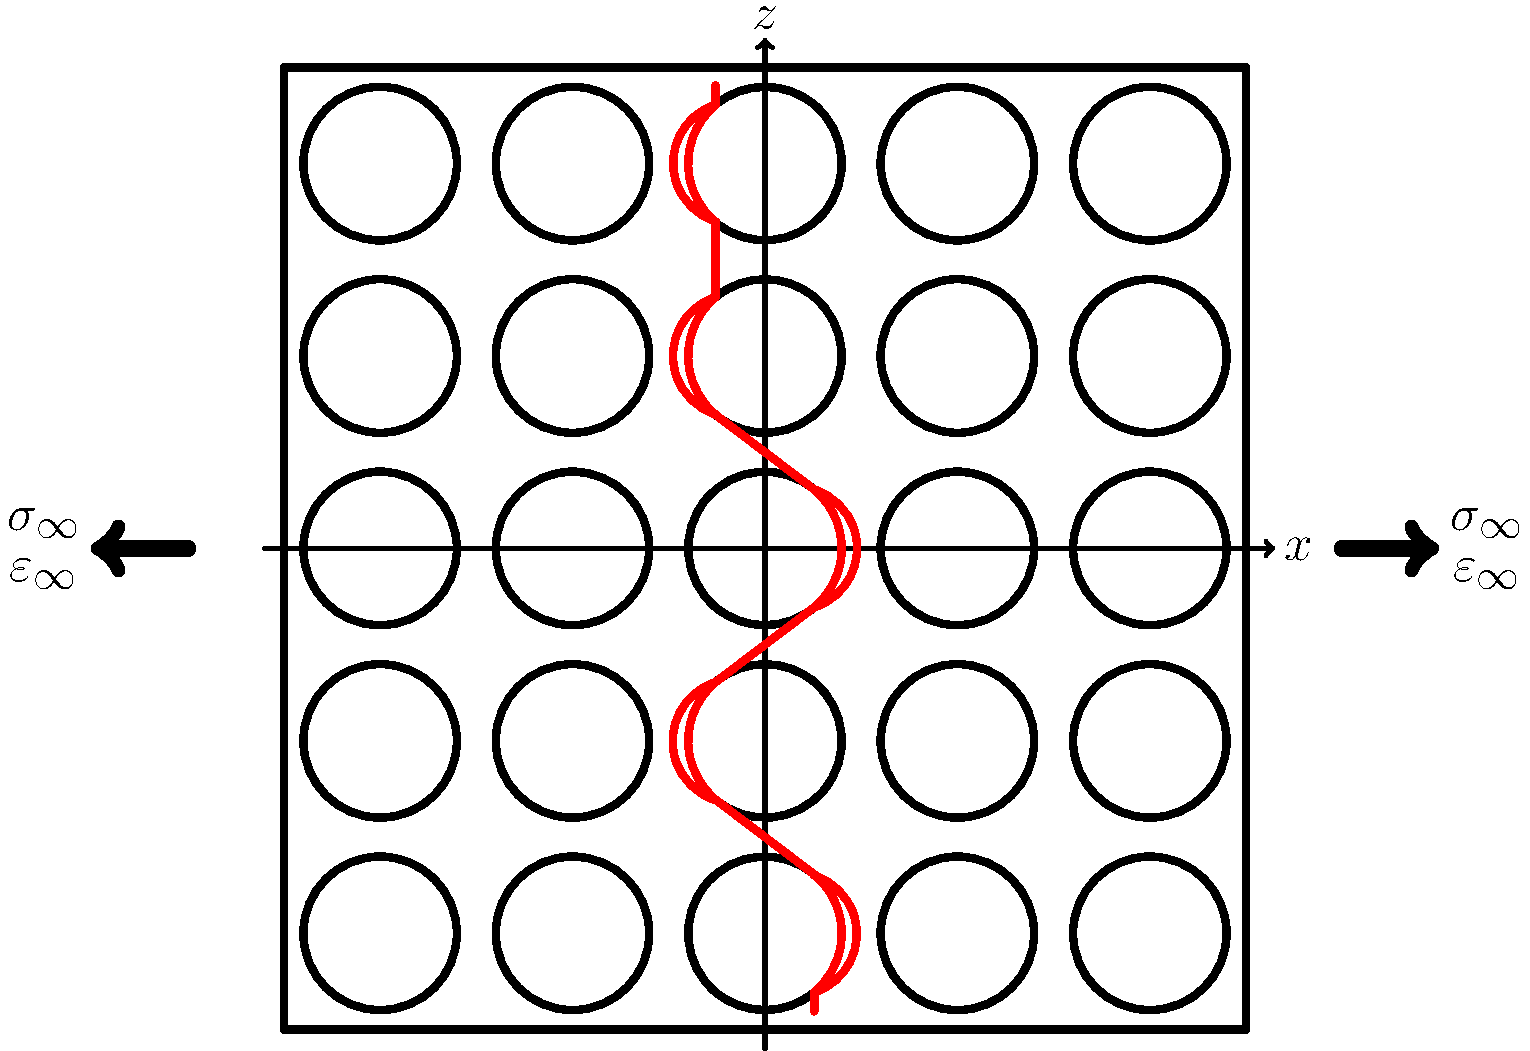
\includegraphics[width=0.6\textwidth]{stage4-coalescence.pdf}
\end{figure}
\end{alertblock}
\vspace{-0.5cm}
%{\tiny J. E. Bailey, P. T. Curtis, A. Parvizi, 1979. {\em\tiny On the transverse cracking and longitudinal splitting behaviour of glass and carbon fibre reinforced epoxy cross ply laminates and the effect of Poisson and thermally generated strain}. {\it\tiny P. Roy. Soc. A-Math. Phy.} {\bf\tiny 366} (1727) pp. 599--623.}
%{\tiny Bailey, J. E., Parvizi, A.; 1981. {\em\tiny On fibre debonding effects and the mechanism of transverse-ply failure in cross-ply laminates of glass fibre/thermoset composites}. {\it\tiny J. Mater. Sci.} {\bf\tiny 16} (3) pp. 649--659.}
{\tiny Zhang, H., Ericson, M. L., Varna, J., Berglund, L.A.; 1997. {\em\tiny Transverse single-fibre test for interfacial debonding in composites: 1. Experimental observations}. {\it\tiny Compos. Part A-Appl. S.} {\bf\tiny 28} (4) pp. 309--315.}
\end{frame}

%
%
%\subsection[Geometry]{The Fiber-Matrix Interface Crack Problem: Geometry}
%
%\begin{frame}
%\frametitle{\small The Fiber-Matrix Interface Crack Problem: Geometry}
%\vspace{-1cm}
%\centering
%\begin{columns}[c]
%\begin{column}{0.85\textwidth}
%\begin{figure}
%\centering
%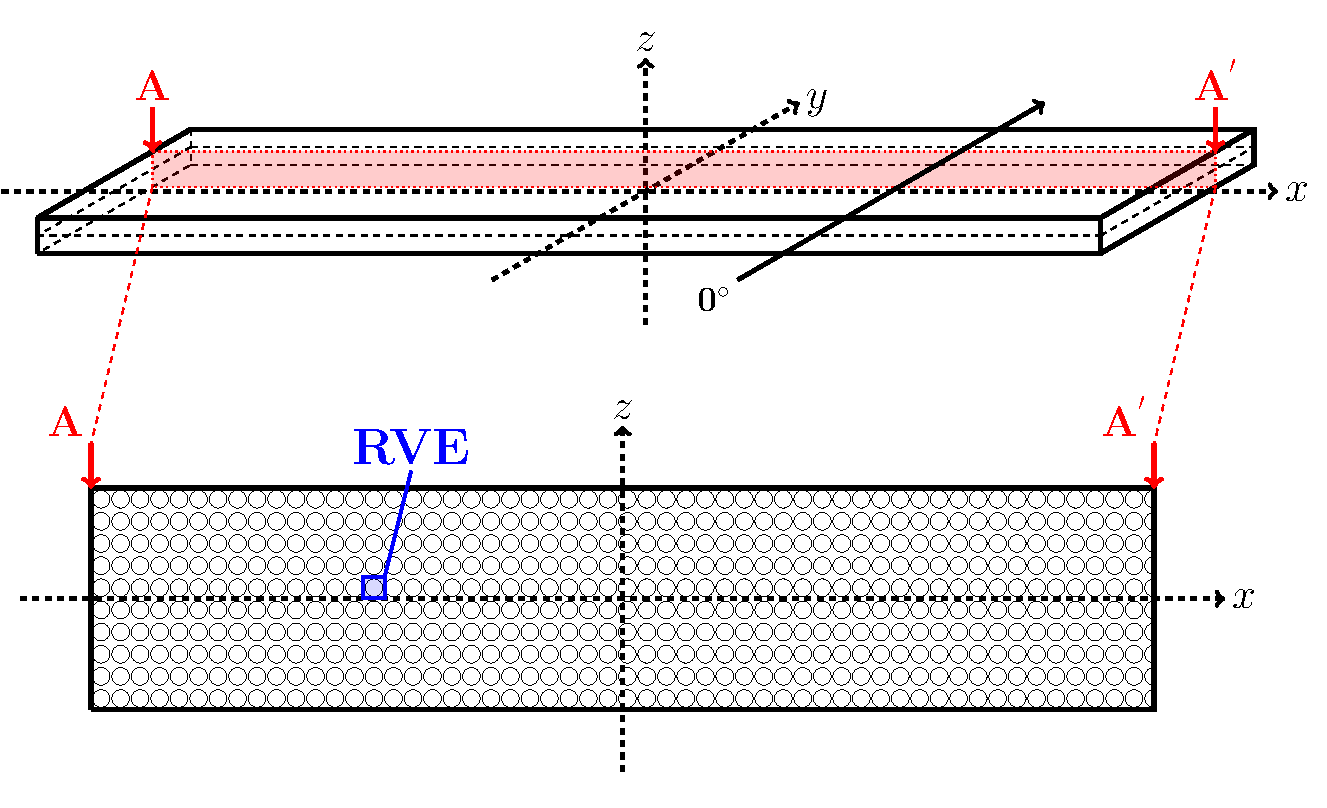
\includegraphics[width=\columnwidth]{laminate-section.pdf}
%\end{figure}
%\end{column}
%\begin{column}{0.15\textwidth}
%\scriptsize
%\begin{itemize}[label=\ding{212}]
%\item $L, W >> t$
%\item $L, W \rightarrow \infty$
%\item Square packing
%\item$L_{d} >> \Delta\theta_{d}$
%\item 2D RVE
%\end{itemize}
%\end{column}
%\end{columns}
%
%\end{frame}
%
%\subsection[Assumptions]{The Fiber-Matrix Interface Crack Problem: Assumptions}
%
%\begin{frame}
%\frametitle{\vspace{0.3cm}\small The Fiber-Matrix Interface Crack Problem: Assumptions}
%\vspace{-1.cm}
%\centering
%\begin{columns}
%\begin{column}{0.6\textwidth}
%\begin{figure}
%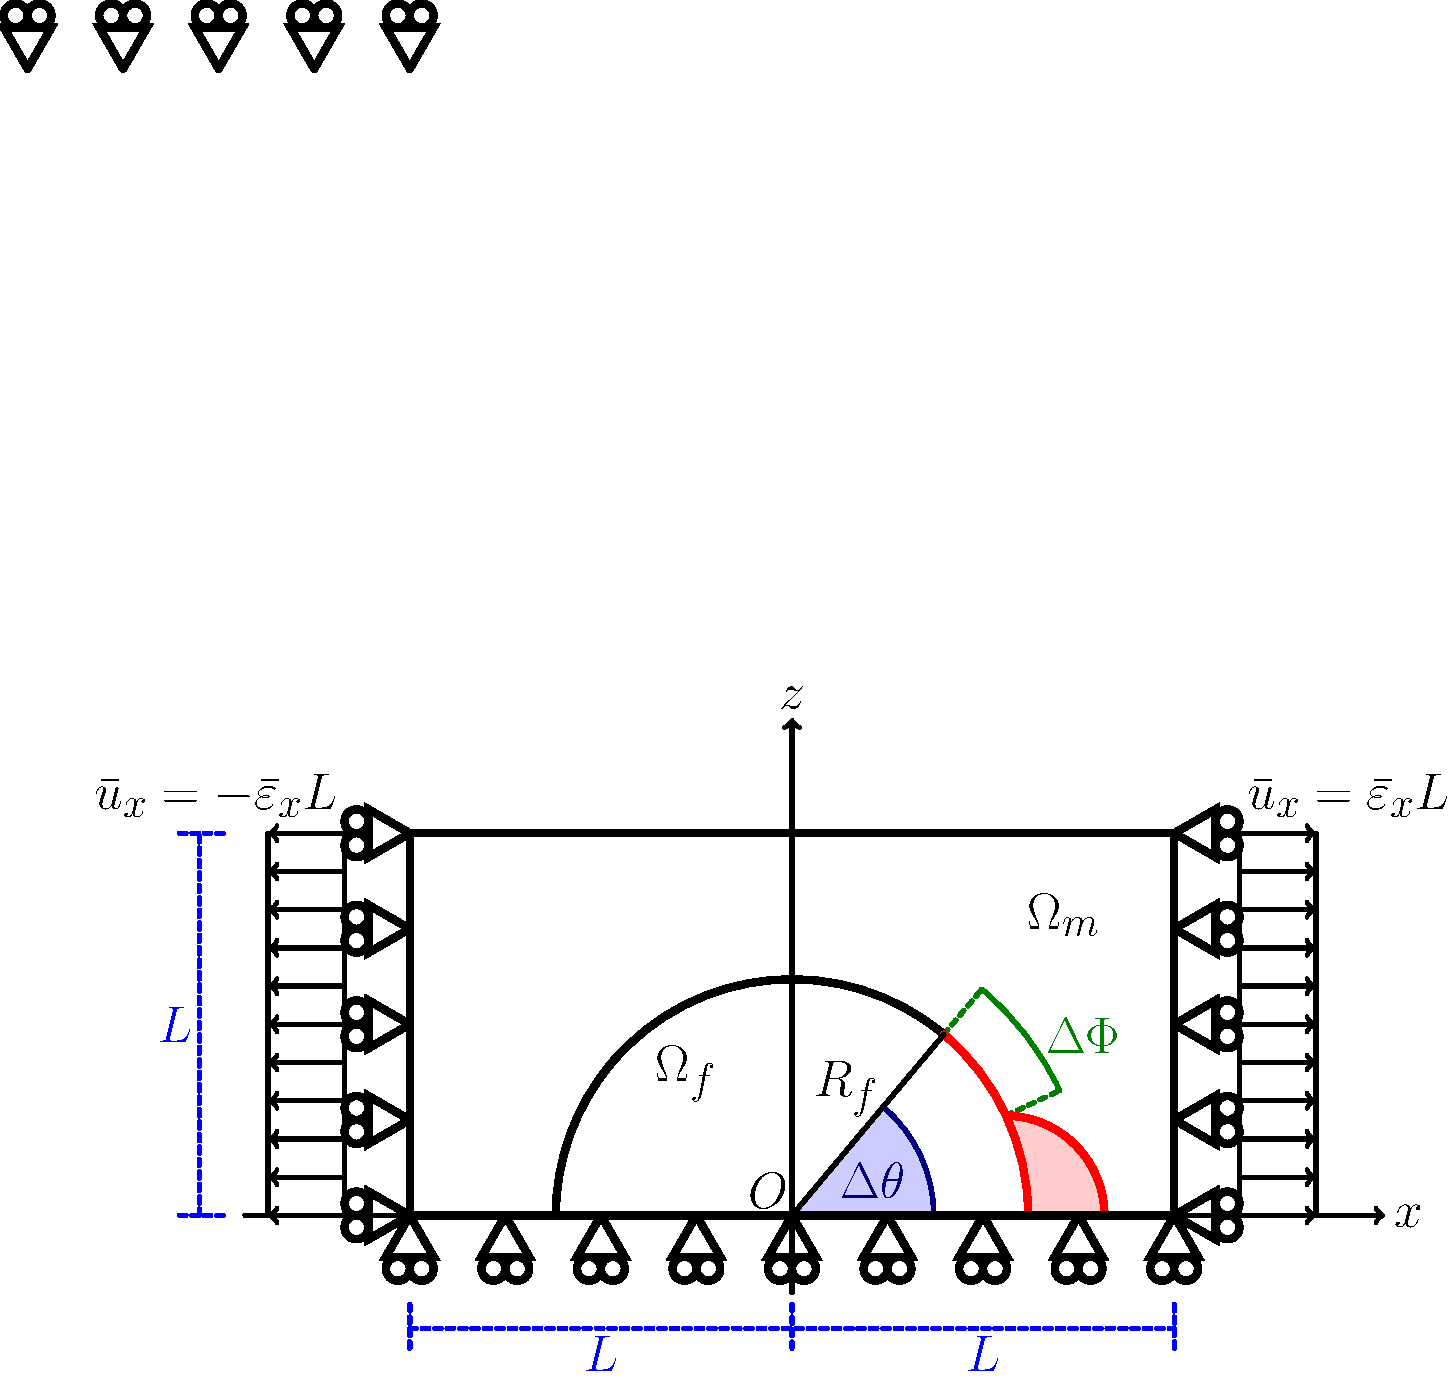
\includegraphics[width=0.95\columnwidth]{RUC.pdf}
%\end{figure}
%\vspace{-0.1cm}
%\scriptsize
%\begin{equation*}
%R_{f}=1\ \left[\mu m\right]\quad L=\frac{R_{f}}{2}\sqrt{\frac{\pi}{V_{f}}}
%\end{equation*}
%\vspace{-0.25cm}
%\begin{table}[htbp]
%\scriptsize
%  \centering
%    \begin{tabular}{ccc}
%    \toprule
%    \textbf{Material} & $\mathbf{E}$ &$\mathbf{\nu}$ \\
%    \midrule
%    glass fiber    & 70.0  & 0.2\\
%    epoxy    & 3.5    & 0.4\\
%    \bottomrule
%    \end{tabular}
%\end{table}
%\end{column}
%\begin{column}{0.4\textwidth}
%\scriptsize
%\begin{itemize}[label=\ding{212}]
%\item Linear elastic, homogeneous and isotropic materials
%\item Plane strain
%\item Frictionless contact interaction
%\item Symmetric w.r.t. x-axis
%\item Coupling of x-displacements on left and right side (repeating unit cell)
%\item Applied uniaxial tensile strain $\bar{\varepsilon}_{x}=1\%$
%\end{itemize}
%\end{column}
%\end{columns}
%\end{frame}
%
%\subsection[Solution]{The Fiber-Matrix Interface Crack Problem: Solution}
%
%\begin{frame}
%\frametitle{\vspace{0.4cm}\small The Fiber-Matrix Interface Crack Problem: Solution}
%\vspace{-1.cm}
%\centering
%\begin{columns}
%\begin{column}{0.6\textwidth}
%\begin{figure}
%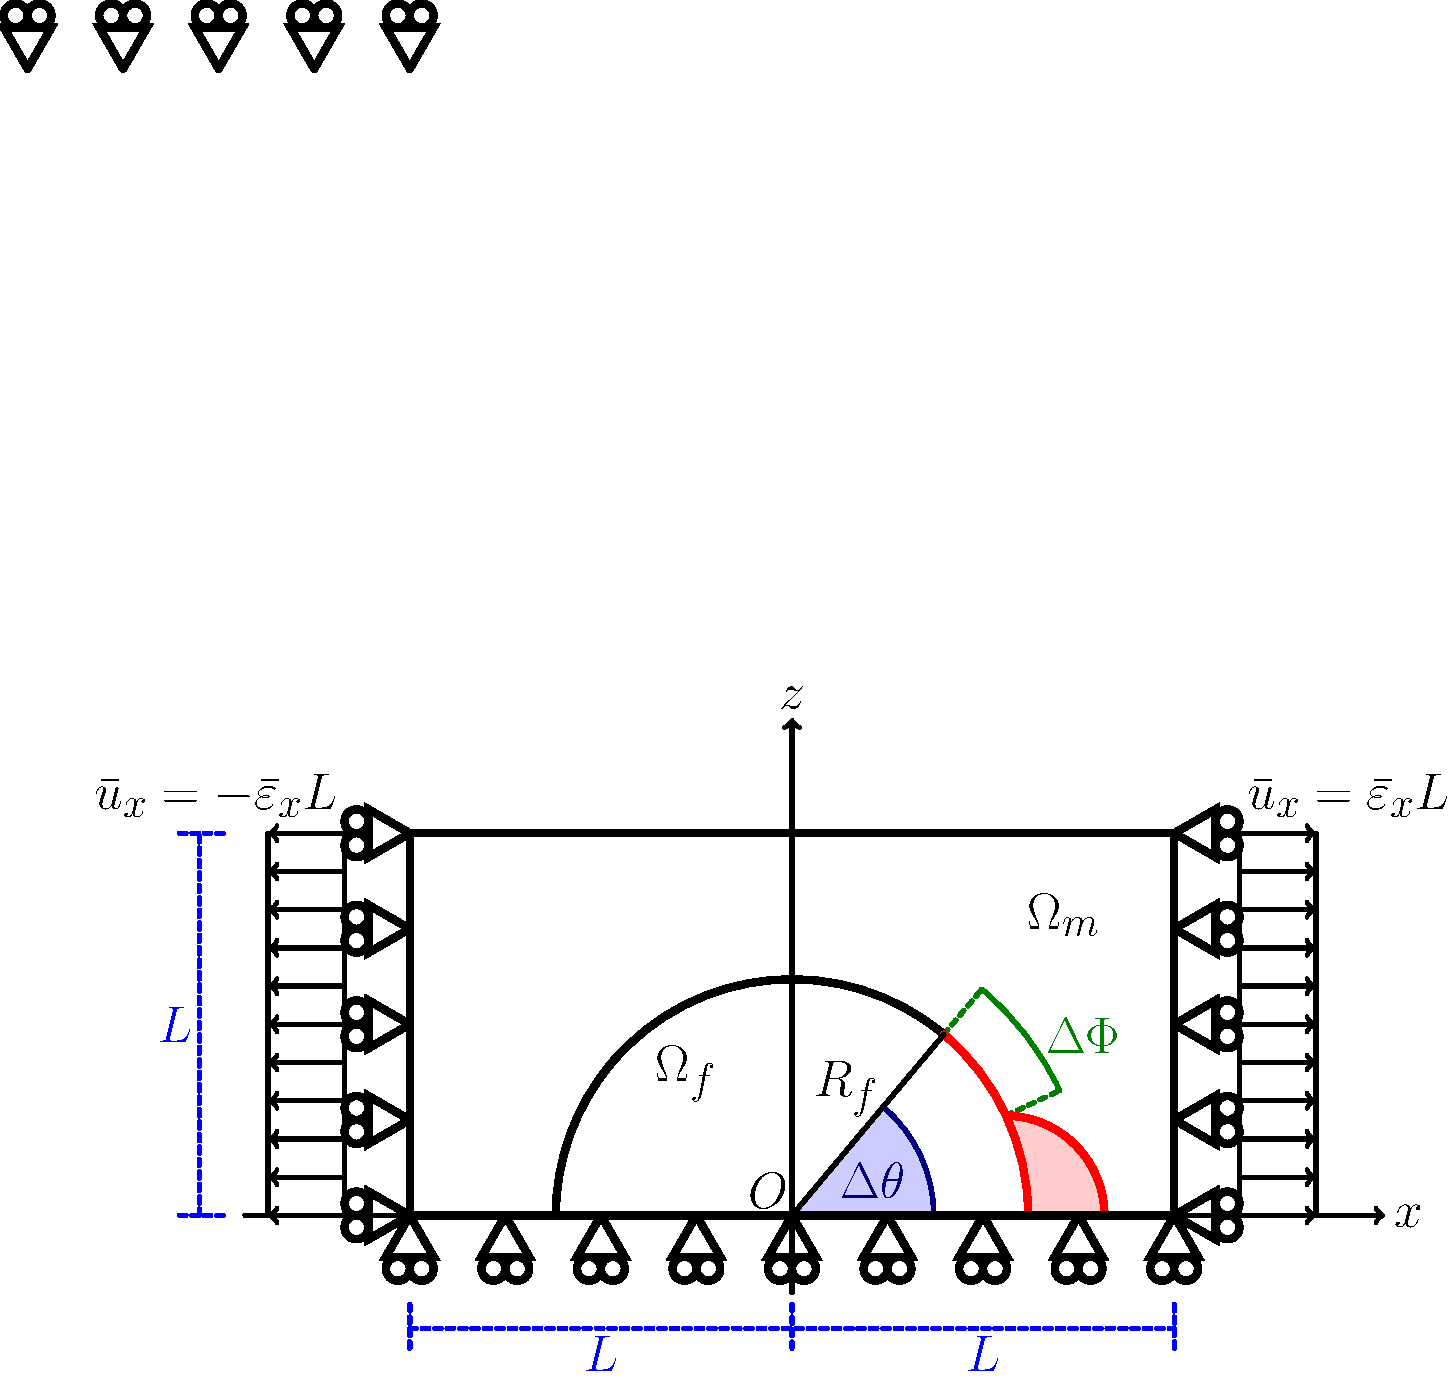
\includegraphics[width=0.95\columnwidth]{RUC.pdf}
%\end{figure}
%\vspace{-0.75cm}
%\begin{columns}
%\begin{column}{0.4\columnwidth}
%\tiny
%\begin{equation*}
%\begin{aligned}
%&\text{in }\Omega_{f}, \Omega_{m}:\\
%&\frac{\partial^{2}\varepsilon_{xx}}{\partial y^{2}}+\frac{\partial^{2}\varepsilon_{yy}}{\partial x^{2}}=\frac{\partial^{2}\gamma_{xy}}{\partial x\partial y}\\
%&\varepsilon_{z}=\gamma_{zx}=\gamma_{yz}=0\\
%&\frac{\partial\sigma_{xx}}{\partial x}+\frac{\partial\tau_{xy}}{\partial y} = 0\\
%&\frac{\partial\tau_{xy}}{\partial x}+\frac{\partial\sigma_{yy}}{\partial y} = 0\\
%&\sigma_{zz}=\nu\left(\sigma_{xx}+\sigma_{yy}\right)\\
%\end{aligned}
%\end{equation*}
%\end{column}
%\begin{column}{0.6\columnwidth}
%\tiny
%\begin{equation*}
%\begin{aligned}
%&\text{for } 0^{\circ}\leq\alpha\leq\Delta\theta:\\
%&\left(\overrightarrow{u}_{m}\left(R_{f},\alpha\right)-\overrightarrow{u}_{f}\left(R_{f},\alpha\right)\right)\cdot\overrightarrow{n}_{\alpha}\geq 0\\
%&\text{for } \Delta\theta\leq\alpha\leq 180^{\circ}:\\
%&\overrightarrow{u}_{m}\left(R_{f},\alpha\right)-\overrightarrow{u}_{f}\left(R_{f},\alpha\right)=0\\
%&\sigma_{ij}=E_{ijkl}\varepsilon_{kl}\\
%&+BC
%\end{aligned}
%\end{equation*}
%\end{column}
%\end{columns}
%\end{column}
%\begin{column}{0.3\textwidth}
%\scriptsize
%\begin{itemize}[label=\ding{212}]
%\item Oscillating singularity
%\vspace{-0.25cm}
%\begin{equation*}
%\sigma\sim r^{-\frac{1}{2}}\sin\left(\varepsilon\log r\right),\quad V_{f}\rightarrow 0
%\end{equation*}
%\vspace{-0.25cm}
%{\tiny
%\begin{equation*}
%\varepsilon=\frac{1}{2\pi}\log\left(\frac{1-\beta}{1+\beta}\right)
%\end{equation*}
%\vspace{-0.25cm}
%\begin{equation*}
%\beta=\frac{\mu_{2}\left(\kappa_{1}-1\right)-\mu_{1}\left(\kappa_{2}-1\right)}{\mu_{2}\left(\kappa_{1}+1\right)+\mu_{1}\left(\kappa_{2}+1\right)}
%\end{equation*}}
%\item Finite Element Method (FEM) in Abaqus\texttrademark
%\item $2^{nd}$ order shape functions
%\item 6-nodes triangles \& 8-nodes quadrilaterals
%\item regular mesh of quadrilaterals at the crack tip:
%\begin{itemize}[label=-]
%\item $AR\sim 1$
%\item $\delta=0.05^{\circ}$
%\end{itemize}
%\end{itemize}
%\end{column}
%\end{columns}
%\end{frame}
%
%\subsection[Normalization \& Scaling]{The Fiber-Matrix Interface Crack Problem: Normalization \& Scaling}
%
%\begin{frame}
%\frametitle{\vspace{0.3cm}\small The Fiber-Matrix Interface Crack Problem: Normalization \& Scaling}
%\vspace{-1.cm}
%\centering
%\begin{columns}[c]
%\begin{column}{0.5\textwidth}
%\begin{figure}
%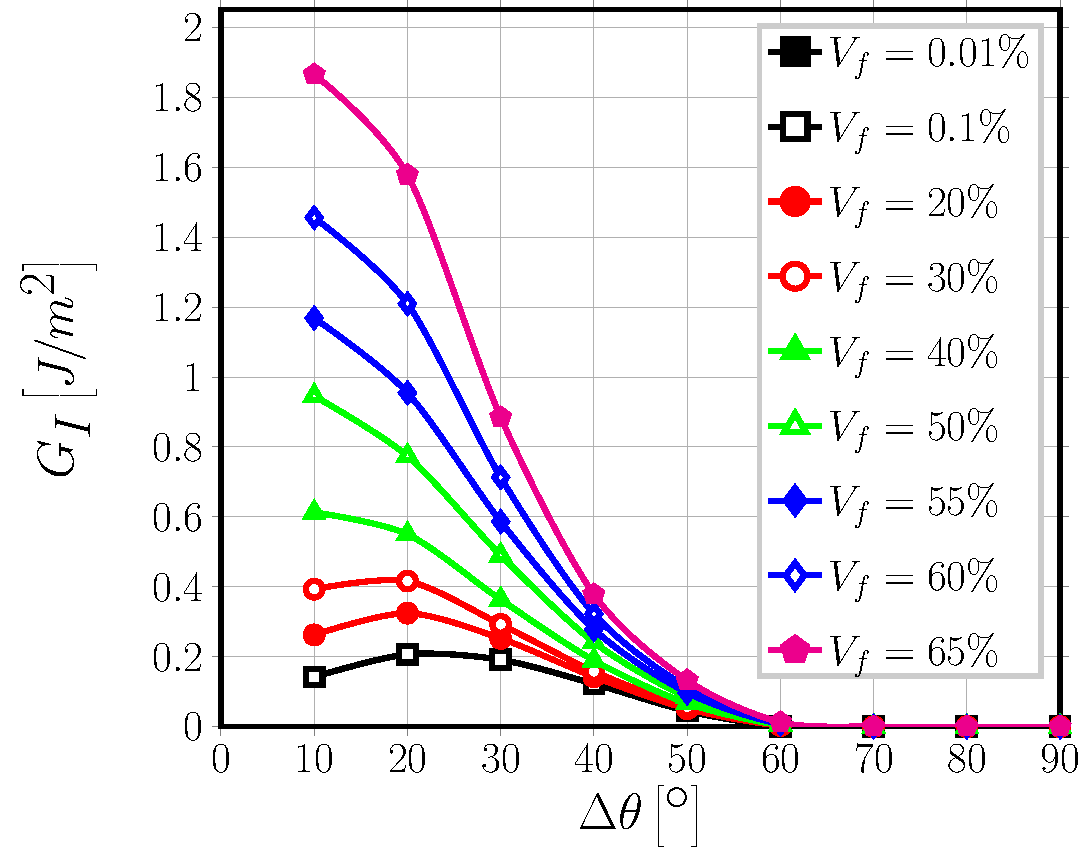
\includegraphics[width=\columnwidth]{GI-free-dim.pdf}
%\end{figure}
%\end{column}
%\begin{column}{0.5\textwidth}
%\begin{figure}
%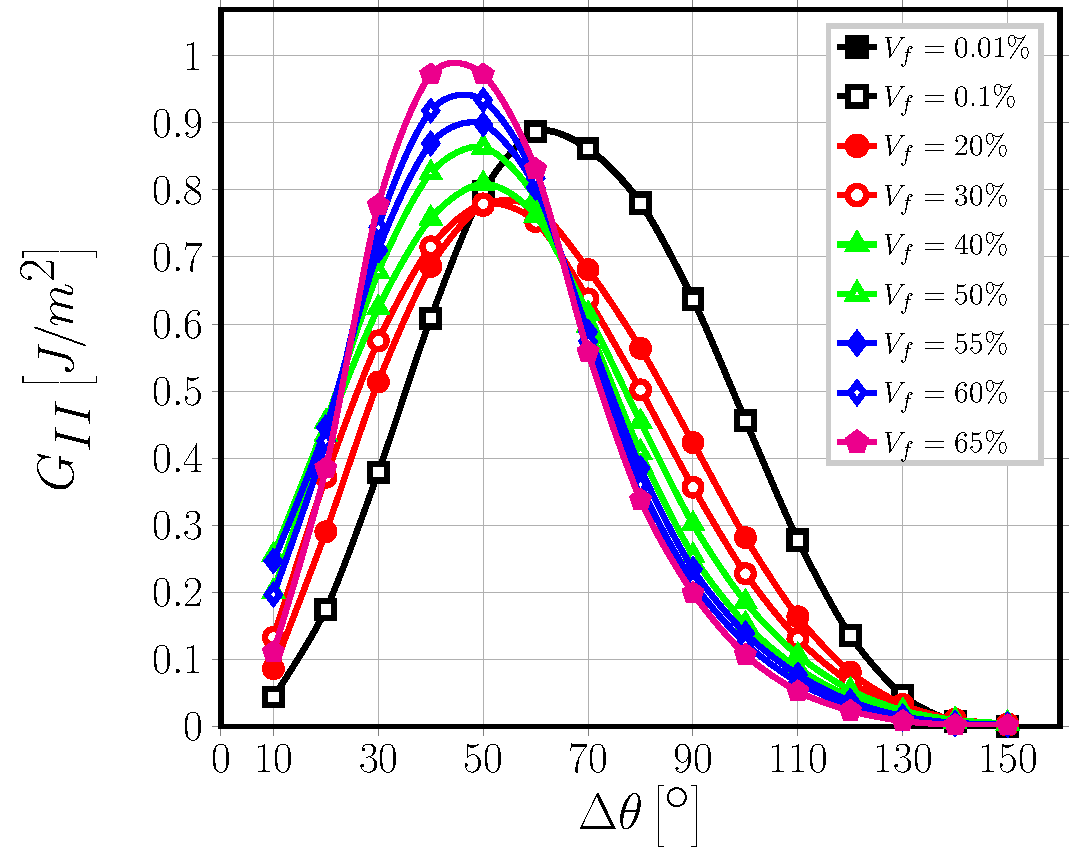
\includegraphics[width=\columnwidth]{GII-free-dim.pdf}
%\end{figure}
%\end{column}
%\end{columns}
%\centering
%\begin{itemize}[label=(?)]
%\centering
%\footnotesize
%\item $G_{I}=G_{0}\left(V_{f},E_{f},\nu_{f},E_{m},\nu_{m},\bar{\varepsilon}_{x},\Delta\theta\right)g_{I}\left(\Delta\theta,BC,microstructure,damage\right)$
%\item $G_{II}=G_{0}\left(V_{f},E_{f},\nu_{f},E_{m},\nu_{m},\bar{\varepsilon}_{x},\Delta\theta\right)g_{II}\left(\Delta\theta,BC,microstructure,damage\right)$
%\end{itemize}
%\end{frame}
%
%\section[Investigation of Scaling Laws]{Investigation of Scaling Laws of the Fiber/Matrix Interface Crack}
%
%\subsection{Dimensional Analysis}
%
%\begin{frame}
%\frametitle{\vspace{0.3cm}\small Dimensional Analysis}
%\vspace{-0.75cm}
%\centering
%\tiny
%\begin{itemize}[label=\ding{212}]
%\item From the definition of Energy Release Rate
%\begin{equation*}
%G=\frac{\partial W}{\partial A} - \left(\frac{\partial U}{\partial A}+\frac{\partial E_{k}}{\partial A}\right)\quad\left[\frac{J}{m^{2}}\right]
%\end{equation*}
%\begin{equation*}
%\left[\frac{J}{m^{2}}\right]\longleftrightarrow\frac{E}{L^{2}}=\frac{F\cdot L}{L^{2}}=\frac{F}{L^{2}}\frac{L}{L}\cdot L=\sigma\varepsilon L
%\end{equation*}
%\begin{equation*}
%G_{0}\sim\sigma_{\infty}\varepsilon_{\infty} L_{c}
%\end{equation*}
%\item From the assumption of linear elasticity and uniaxial loading
%\begin{equation*}
%\sigma_{\infty}=E_{eq}\varepsilon_{\infty}\qquad\varepsilon_{\infty}=\frac{\sigma_{\infty}}{E_{eq}}
%\end{equation*}
%\begin{equation*}
%G_{0}\sim E_{eq}\varepsilon^{2}_{\infty}L_{c}\qquad G_{0}\sim\frac{\sigma^{2}_{\infty}}{E_{eq}}L_{c}
%\end{equation*}
%\item From crack geometry
%\begin{equation*}
%L_{c}\sim a=R_{f}\Delta\theta\longrightarrow L_{c}\sim R_{f}f\left(\Delta\theta\right)
%\end{equation*}
%\end{itemize}
%\vspace{-0.25cm}
%\begin{alertblock}{\scriptsize\centering$G_{0}=A\cdot E_{eq}\varepsilon^{2}_{\infty}R_{f}f\left(\Delta\theta\right)$}
%%\scriptsize
%%\centering
%%\begin{equation*}
%%G_{0}=A\cdot E_{eq}\varepsilon^{2}_{\infty}R_{f}f\left(\Delta\theta\right)
%%\end{equation*}
%\end{alertblock}
%\end{frame}
%
%\subsection[Homogenization]{Homogenization of Material Properties}
%
%\begin{frame}
%\frametitle{\vspace{0.35cm}\footnotesize Homogenization of Material Properties: Concentric Cylinders Assembly (CCA)}
%\vspace{-0.75cm}
%\centering
%\tiny
%\begin{equation*}
%E_{L}=V_{f}E_{f}+\left(1-V_{f}\right)E_{m}+2\lambda_{1}\left(\nu_{m}-\nu_{f}\right)^{2}V_{f}\left(1-V_{f}\right)
%\end{equation*}
%\begin{equation*}
%\nu_{LT}=V_{f}\nu_{f}+\left(1-V_{f}\right)\nu_{m}+\frac{\lambda_{1}}{2}\left(\nu_{m}-\nu_{f}\right)\left(\frac{1}{k_{fT}}-\frac{1}{k_{mT}}\right)V_{f}\left(1-V_{f}\right)
%\end{equation*}
%%\begin{equation*}
%%G_{LT}=\frac{E_{m}}{2\left(1+\nu_{m}\right)}+\frac{V_{f}}{\frac{1}{\frac{E_{f}}{2\left(1+\nu_{f}\right)}-\frac{E_{m}}{2\left(1+\nu_{m}\right)}}+\frac{1-V_{f}}{\frac{E_{m}}{1+\nu_{m}}}}
%%\end{equation*}
%\begin{equation*}
%G_{TT}=\frac{E_{m}}{2\left(1+\nu_{m}\right)}+\frac{V_{f}}{\frac{1}{\frac{E_{f}}{2\left(1+\nu_{f}\right)}-\frac{E_{m}}{2\left(1+\nu_{m}\right)}}+\frac{k_{mT}+\frac{E_{m}}{1+\nu_{m}}}{\frac{E_{m}}{1+\nu_{m}}\left(k_{mT}+\frac{E_{m}}{2\left(1+\nu_{m}\right)}\right)}\left(1-V_{f}\right)}
%\end{equation*}
%\begin{equation*}
%K_{TT}=\frac{k_{mT}\left(k_{fT}+\frac{E_{m}}{2\left(1+\nu_{m}\right)}\right)\left(1-V_{f}\right)+k_{fT}\left(k_{mT}+\frac{E_{m}}{2\left(1+\nu_{m}\right)}\right)V_{f}}{\left(k_{fT}+\frac{E_{m}}{2\left(1+\nu_{m}\right)}\right)\left(1-V_{f}\right)+\left(k_{mT}+\frac{E_{m}}{2\left(1+\nu_{m}\right)}\right)V_{f}}
%\end{equation*}
%\begin{equation*}
%E_{T}=\frac{4G_{TT}}{1+\frac{\left(1+\frac{4K_{TT}\nu_{LT}^{2}}{E_{L}}\right)G_{TT}}{K_{23}}}\qquad\nu_{TT}=\frac{E_{T}}{2G_{TT}}-1
%\end{equation*}
%\begin{equation*}
%k_{fT}=\frac{E_{f}}{2\left(1-\nu_{f}-2\nu_{f}^{2}\right)}\quad k_{mT}=\frac{E_{m}}{2\left(1-\nu_{m}-2\nu_{m}^{2}\right)}\quad\lambda_{1}=2\left(\frac{2\left(1+\nu_{m}\right)}{E_{m}}+\frac{V_{f}}{k_{mT}}+\frac{1-V_{f}}{k_{fT}}\right)^{-1}
%\end{equation*}
%\end{frame}
%
%\begin{frame}
%\frametitle{\small Homogenization of Material Properties: Plane Strain Conditions}
%\vspace{-0.5cm}
%\centering
%\small
%\begin{equation*}
%E_{\text{plane strain}}=\frac{E_{T}}{1-\frac{E_{T}}{E_{L}}\nu_{LT}^{2}}
%\end{equation*}
%\begin{alertblock}{\centering$E_{eq}=\frac{E_{T}}{1-\frac{E_{T}}{E_{L}}\nu_{LT}^{2}}$}
%\end{alertblock}
%\begin{figure}
%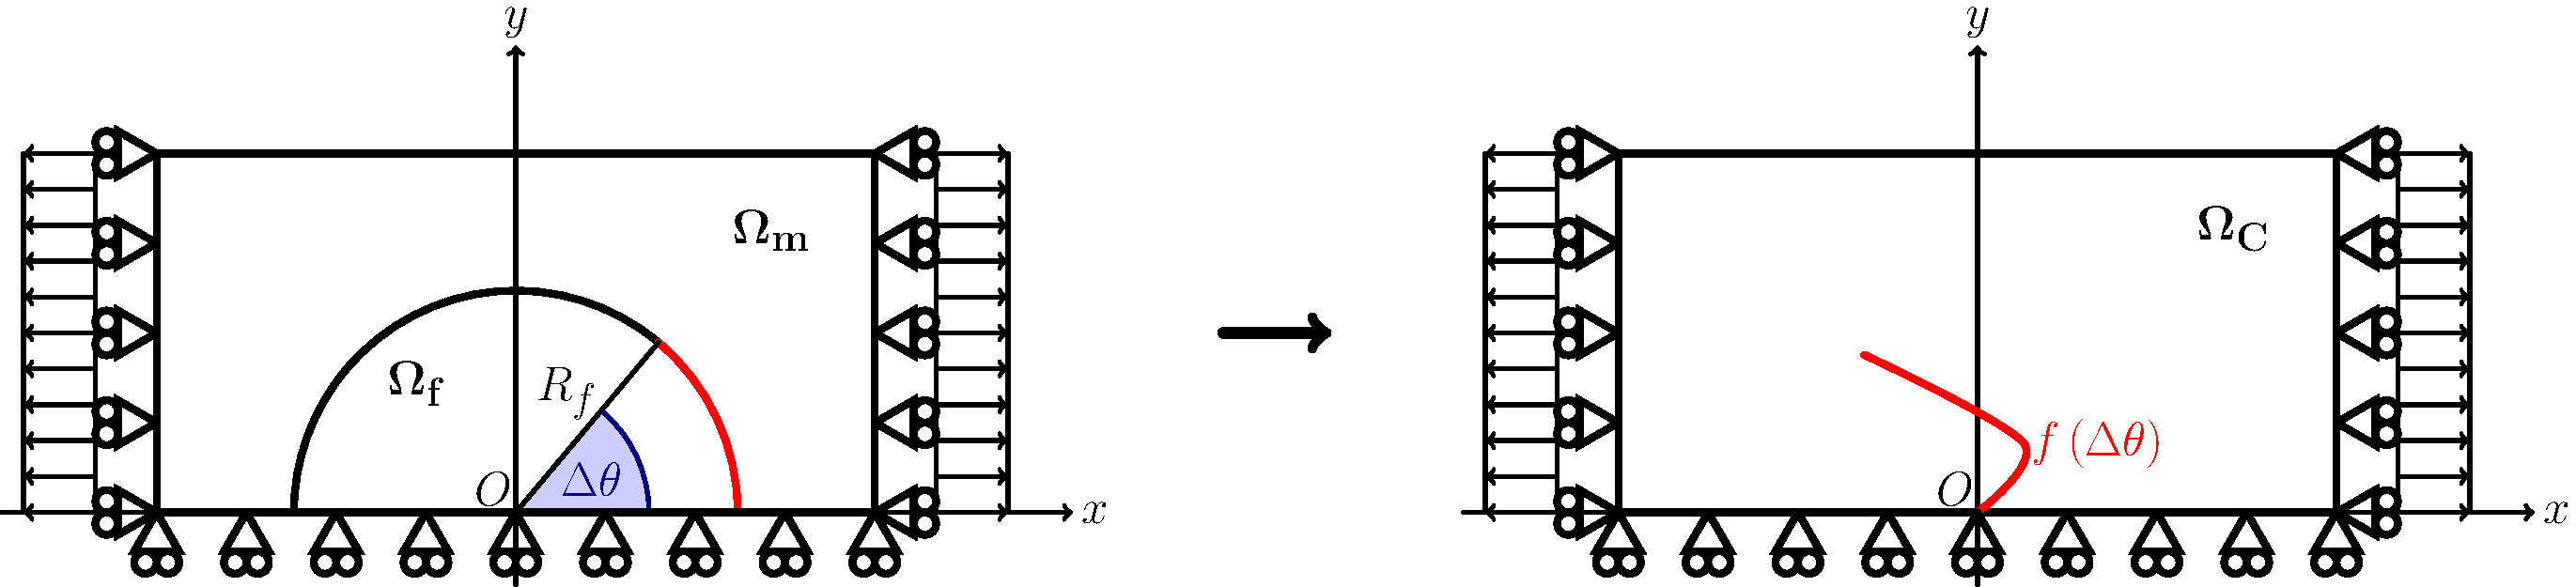
\includegraphics[width=\textwidth]{RUCequivalence.pdf}
%\end{figure}
%\end{frame}
%
%\subsection{Shape Function Reference Configurations}
%
%\begin{frame}
%\frametitle{\vspace{0.4cm}\footnotesize Shape Function Reference Configurations: Straight Crack}
%\vspace{-1.25cm}
%\centering
%\begin{figure}
%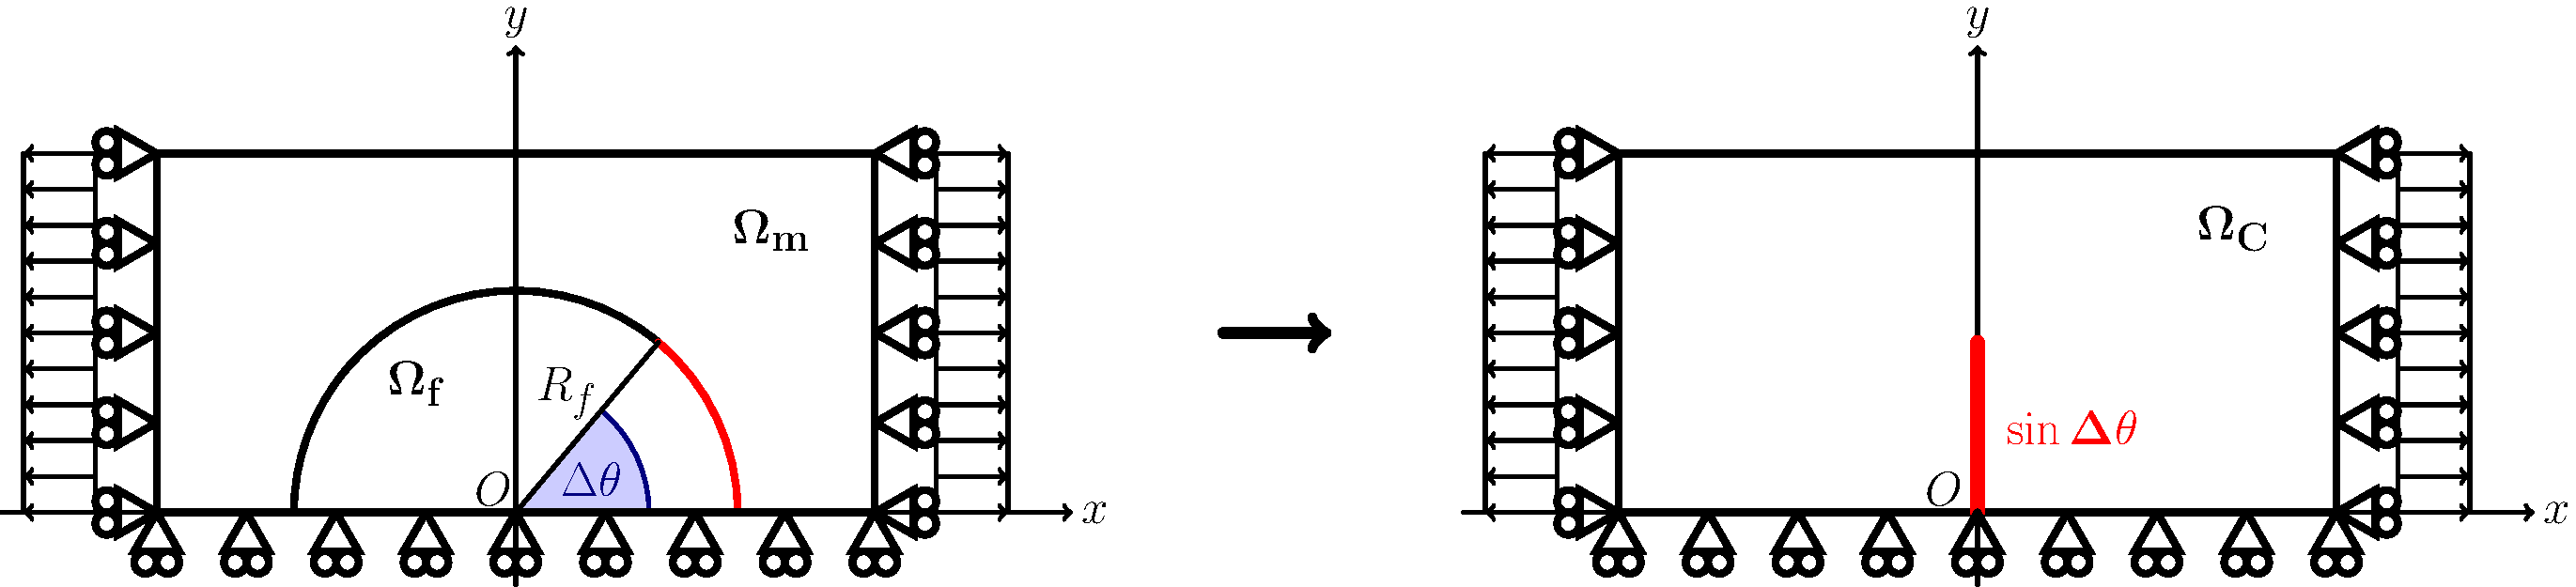
\includegraphics[width=0.9\textwidth]{RUCstraightcrack.pdf}
%\end{figure}
%\vspace{-0.5cm}
%\begin{columns}[c]
%\begin{column}{0.5\textwidth}
%\centering
%\begin{figure}
%\centering
%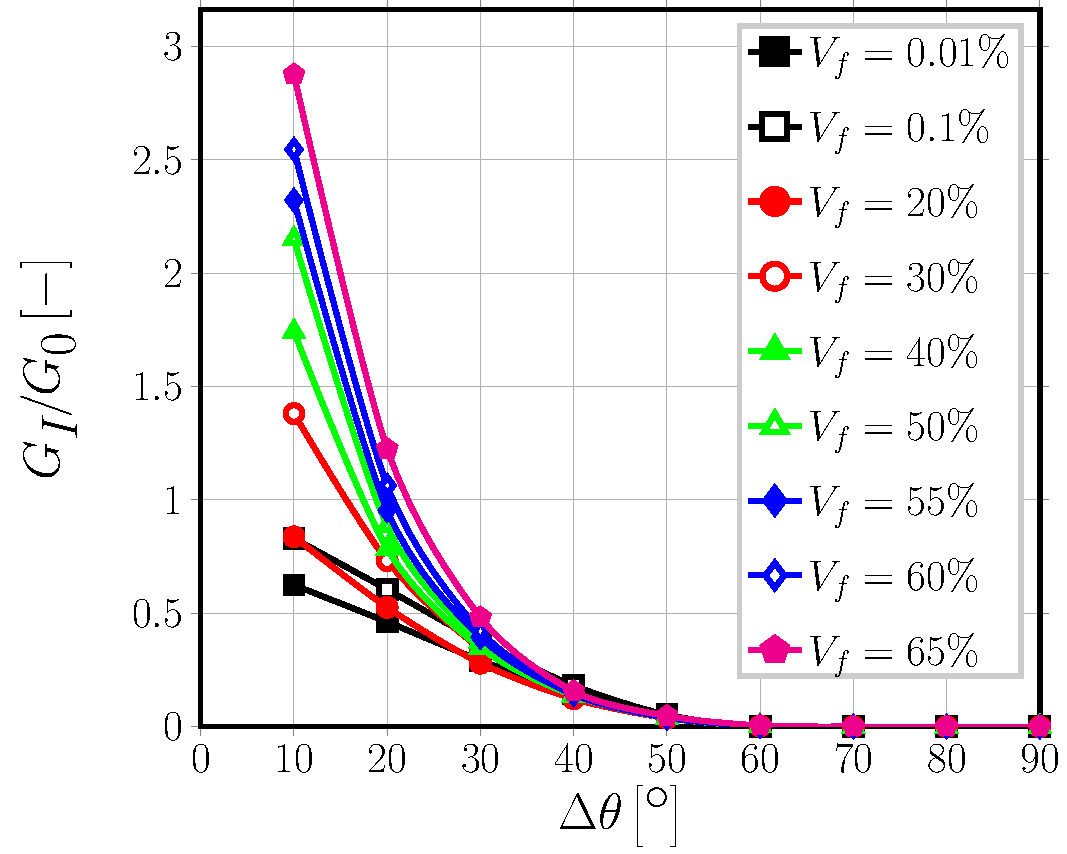
\includegraphics[width=0.9\columnwidth]{GI-free-straightcrack.pdf}
%\end{figure}
%\end{column}
%\begin{column}{0.5\textwidth}
%\centering
%\begin{figure}
%\centering
%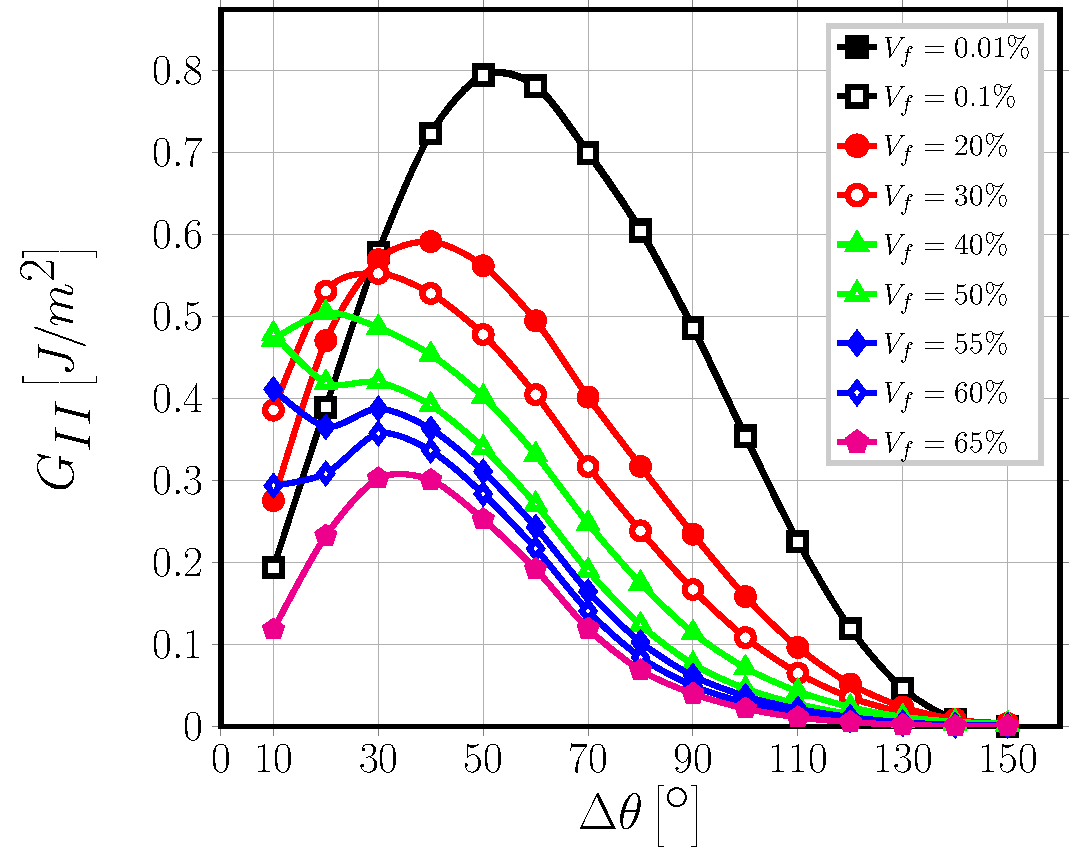
\includegraphics[width=0.9\columnwidth]{GII-free-straightcrack.pdf}
%\end{figure}
%\end{column}
%\end{columns}
%\end{frame}
%
%\begin{frame}
%\frametitle{\vspace{0.4cm}\footnotesize Shape Function Reference Configurations: Inclined Crack}
%\vspace{-1.25cm}
%\centering
%\begin{figure}
%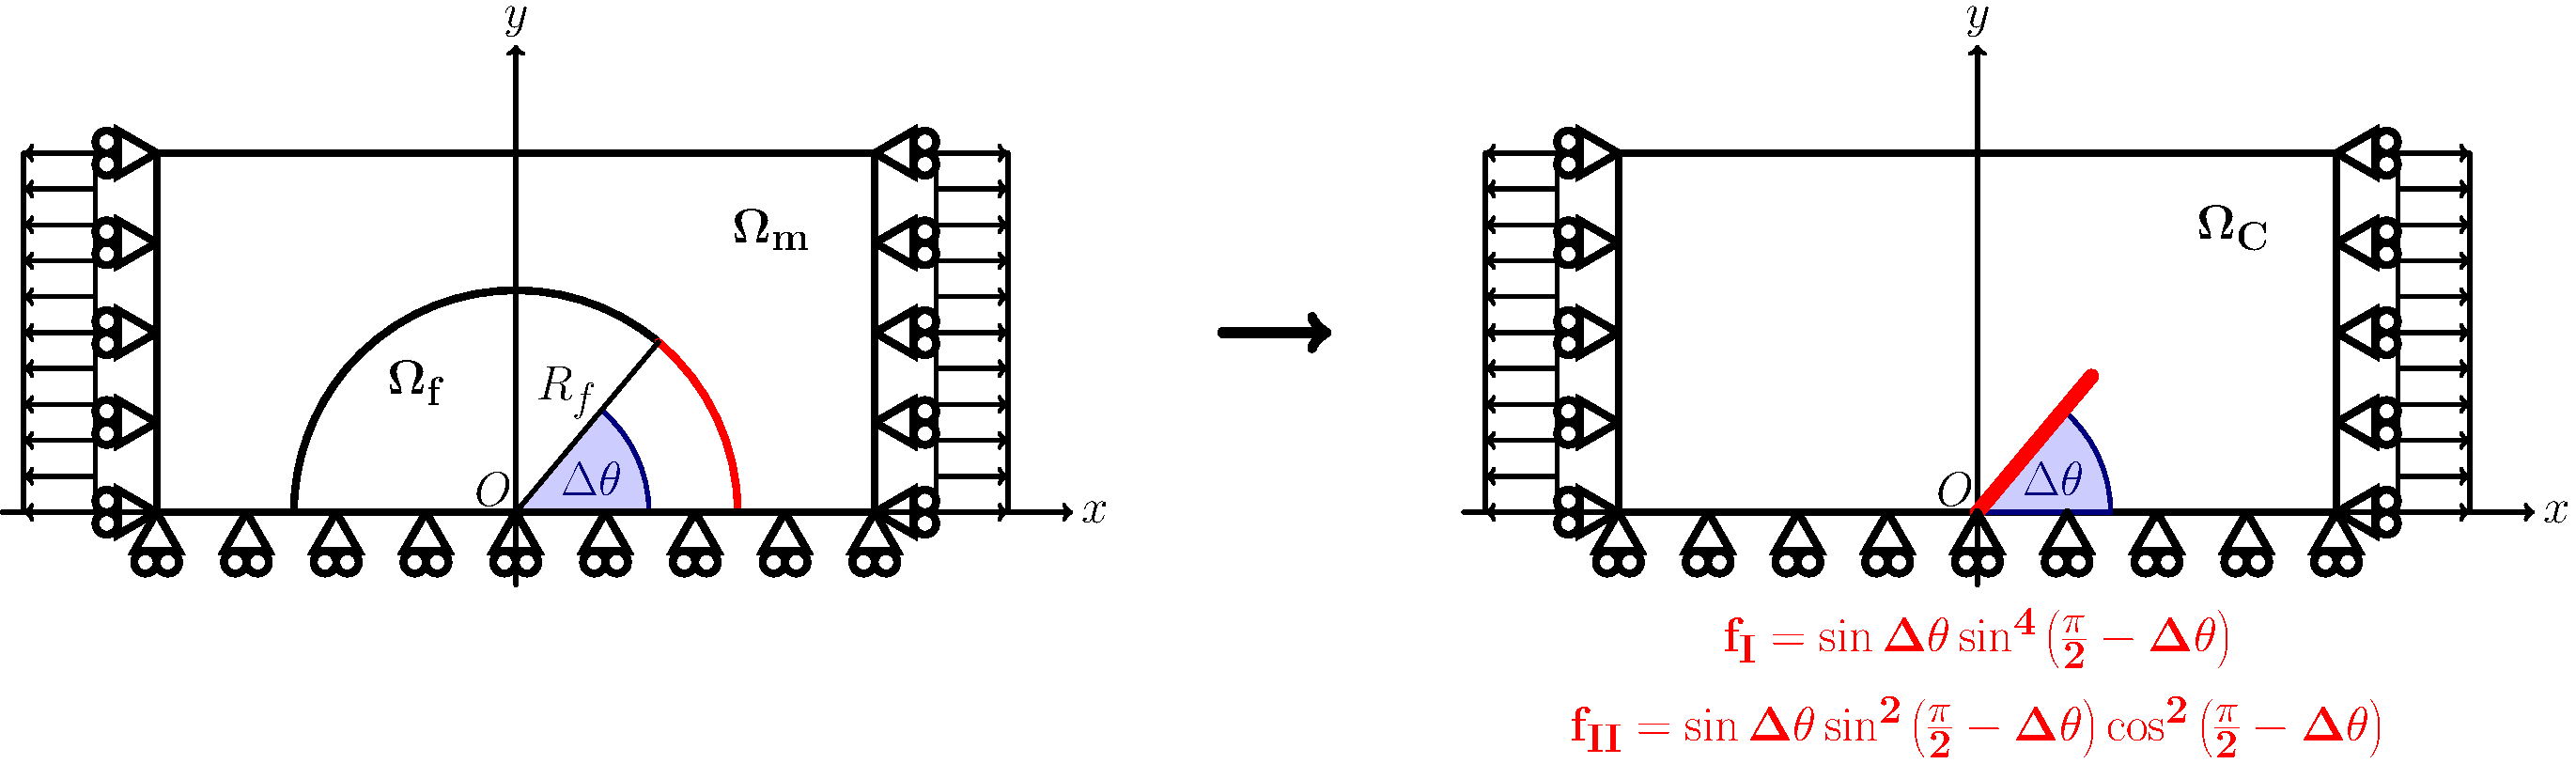
\includegraphics[width=0.9\textwidth]{RUCinclinedcrack.pdf}
%\end{figure}
%\vspace{-0.5cm}
%\begin{columns}[c]
%\begin{column}{0.5\textwidth}
%\centering
%\begin{figure}
%\centering
%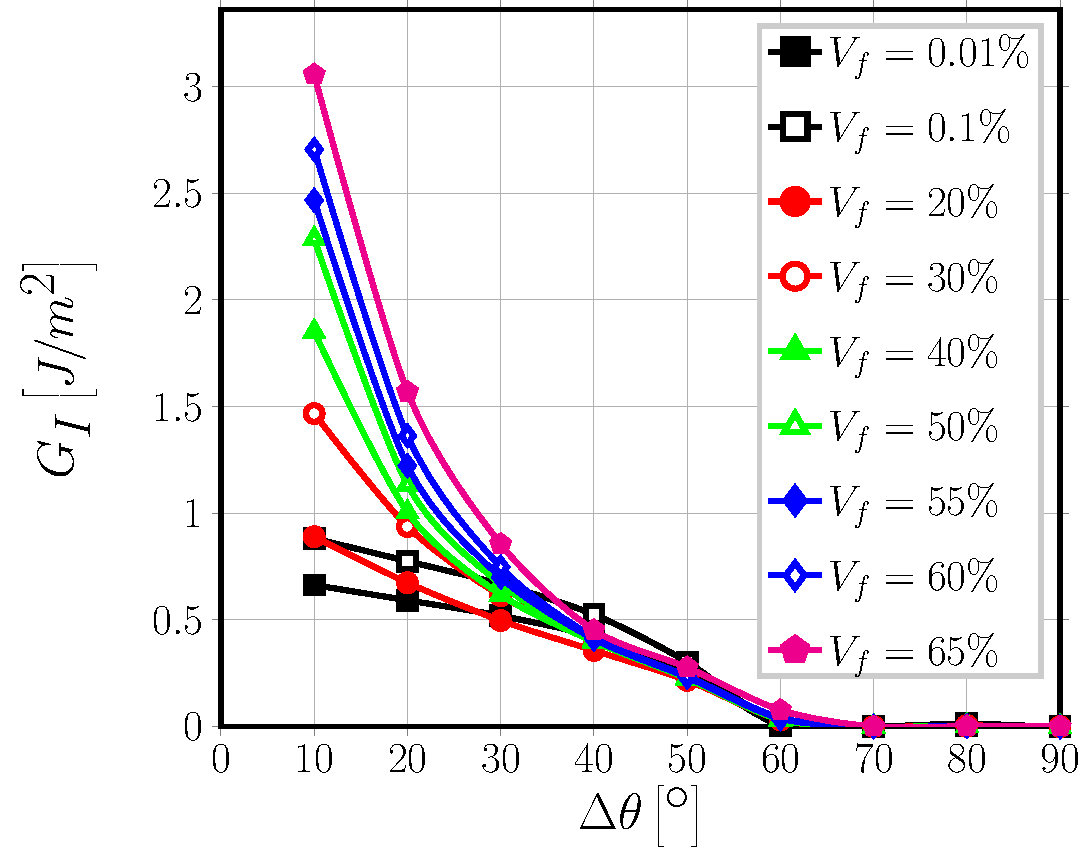
\includegraphics[width=0.9\columnwidth]{GI-free-inclinedcrack.pdf}
%\end{figure}
%\end{column}
%\begin{column}{0.5\textwidth}
%\centering
%\begin{figure}
%\centering
%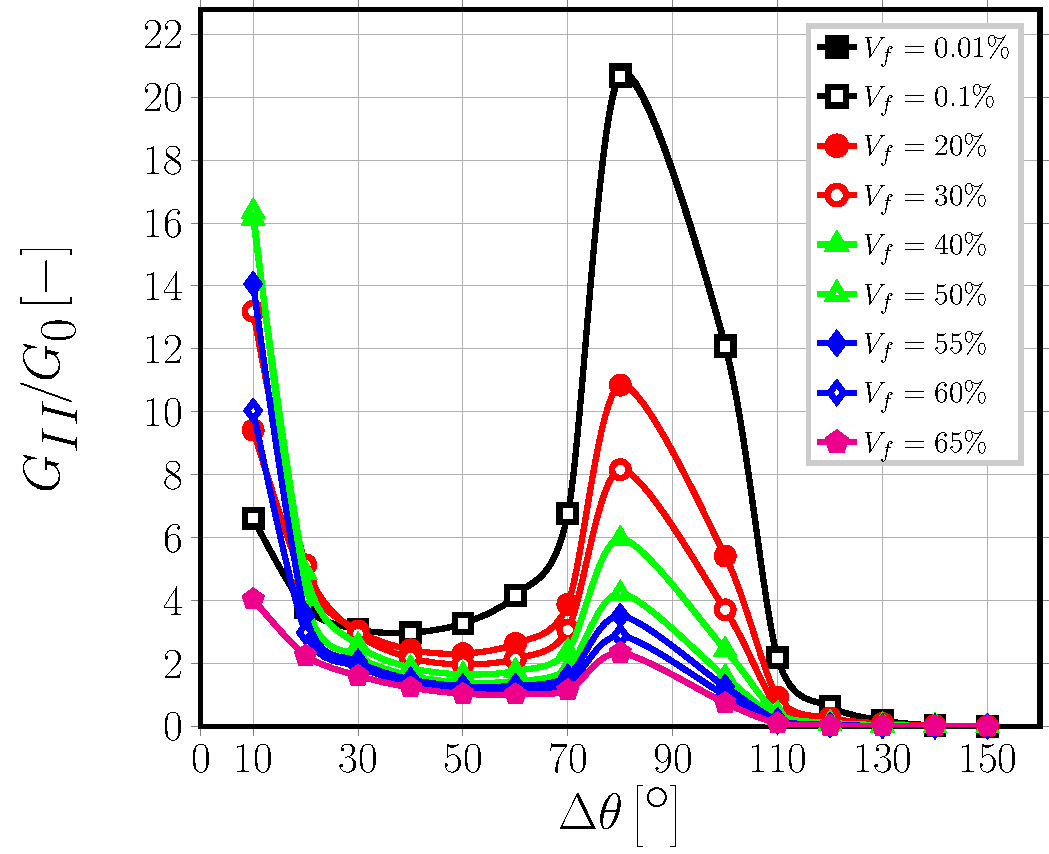
\includegraphics[width=0.9\columnwidth]{GII-free-inclinedcrack.pdf}
%\end{figure}
%\end{column}
%\end{columns}
%\end{frame}
%
%\begin{frame}
%\frametitle{\vspace{0.4cm}\footnotesize Shape Function Reference Configurations: Circular Crack}
%\vspace{-1.25cm}
%\centering
%\begin{figure}
%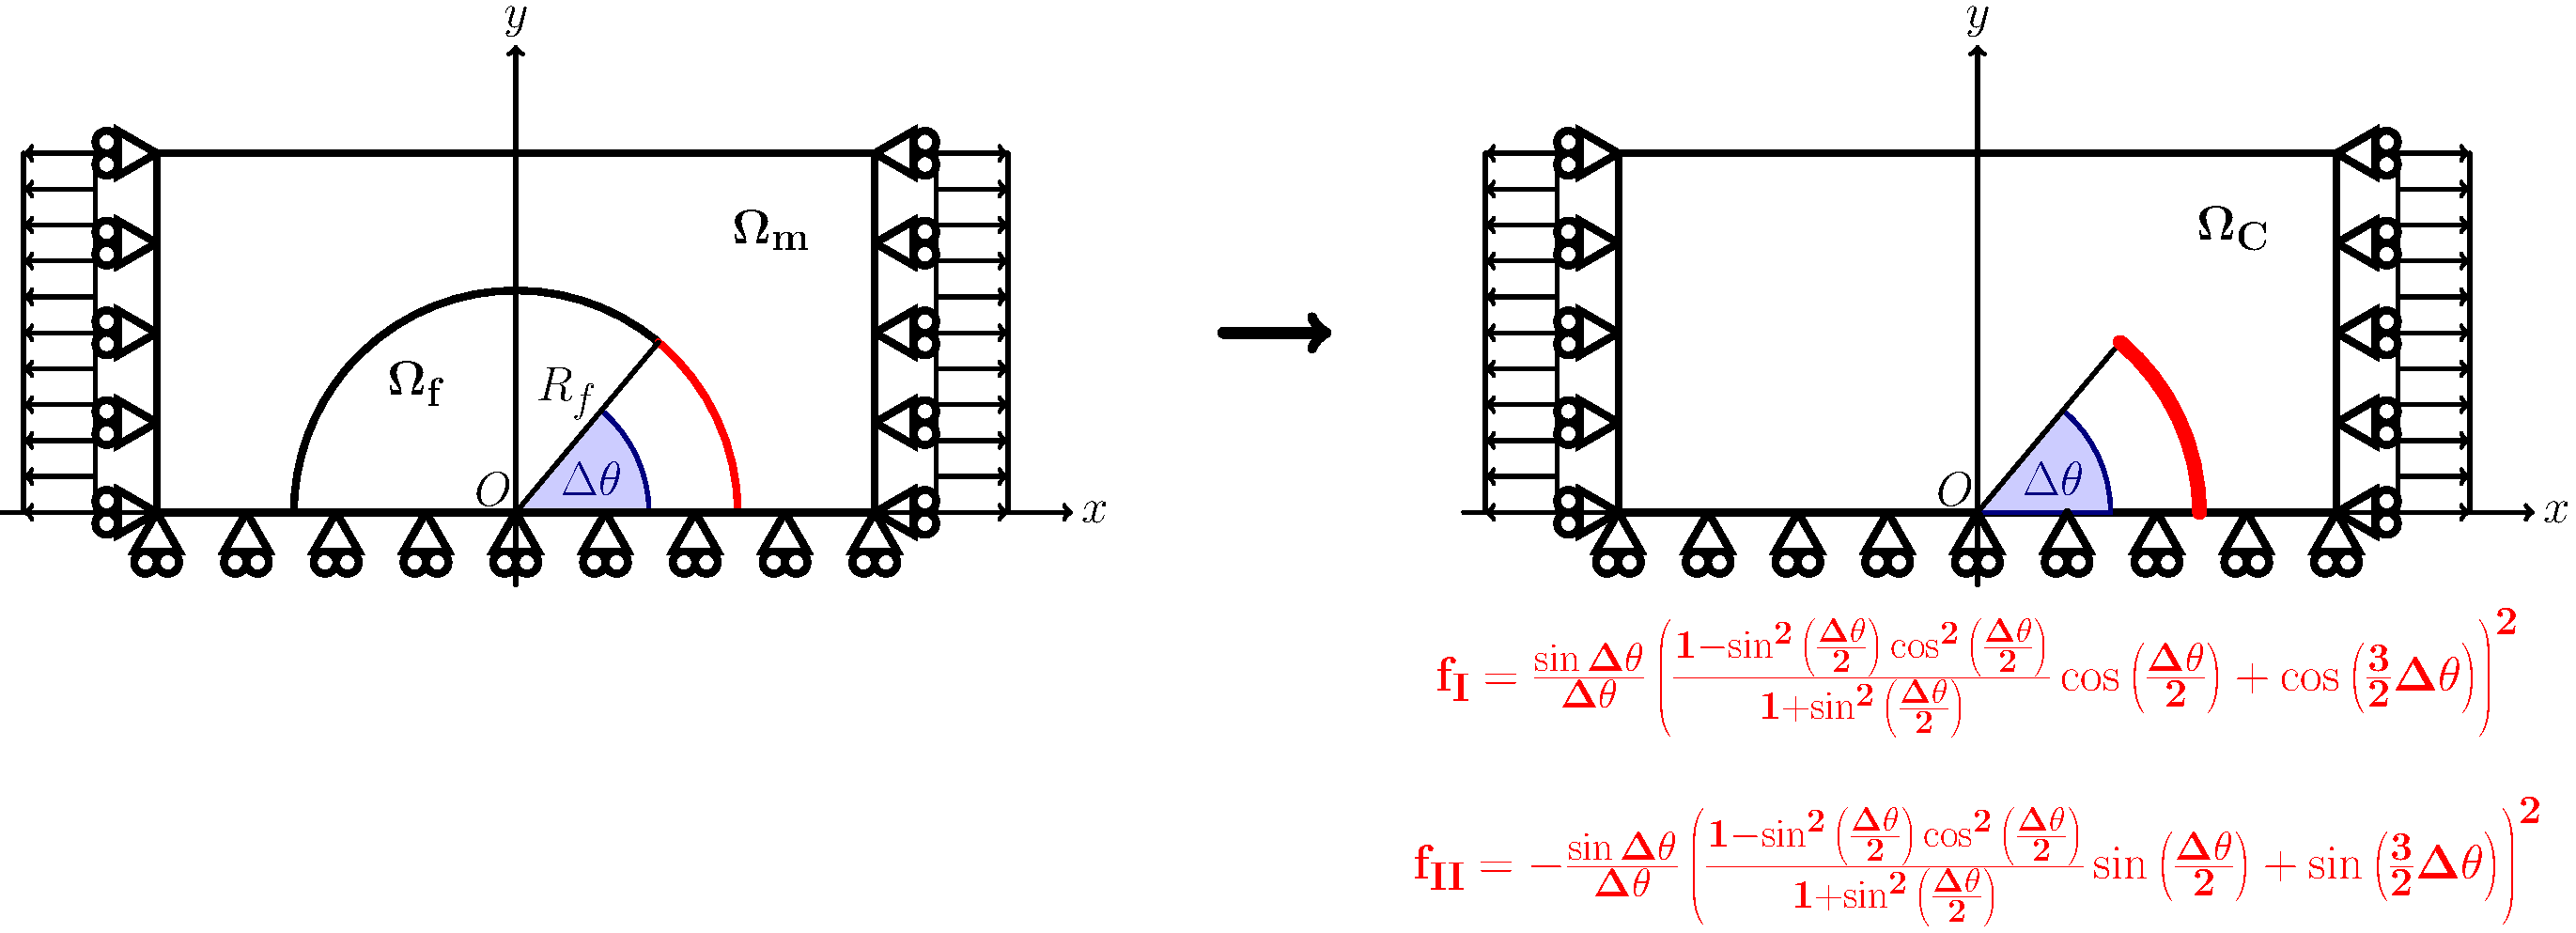
\includegraphics[width=0.9\textwidth]{RUCcurvedcrack.pdf}
%\end{figure}
%\vspace{-0.75cm}
%\begin{columns}[c]
%\begin{column}{0.5\textwidth}
%\centering
%\begin{figure}
%\centering
%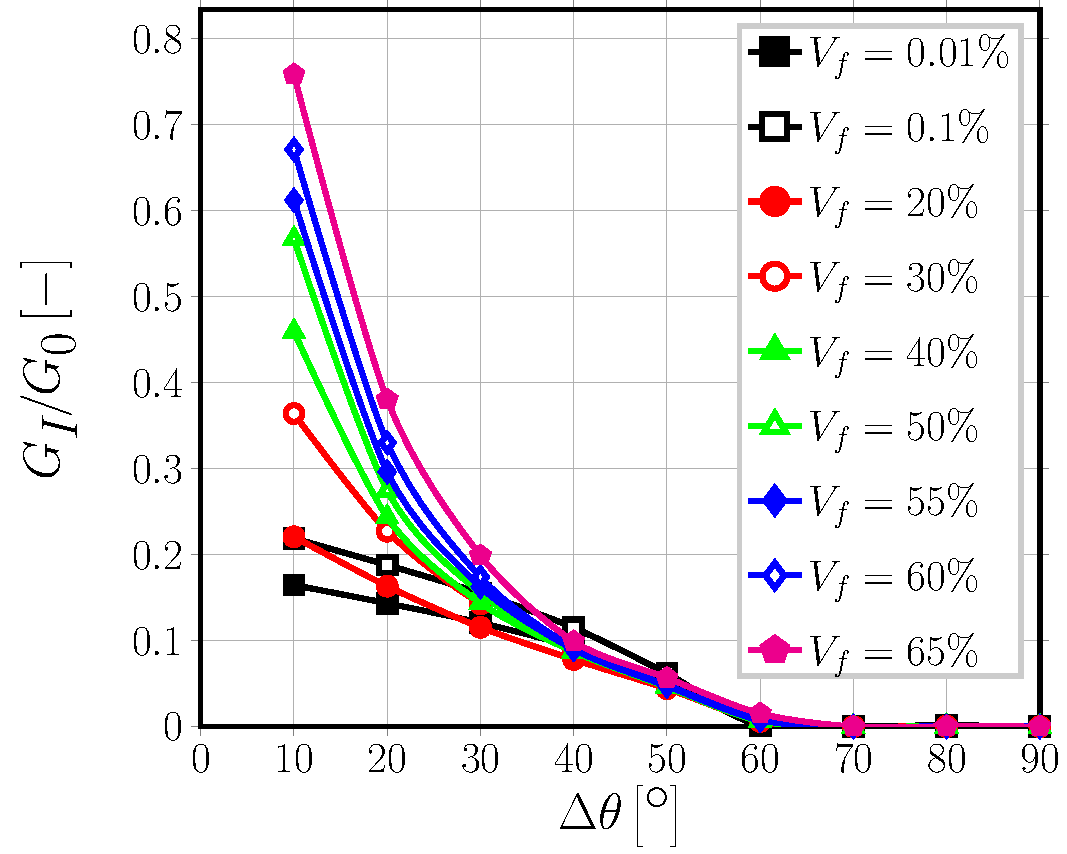
\includegraphics[width=0.9\columnwidth]{GI-free-curvedcrack.pdf}
%\end{figure}
%\end{column}
%\begin{column}{0.5\textwidth}
%\centering
%\begin{figure}
%\centering
%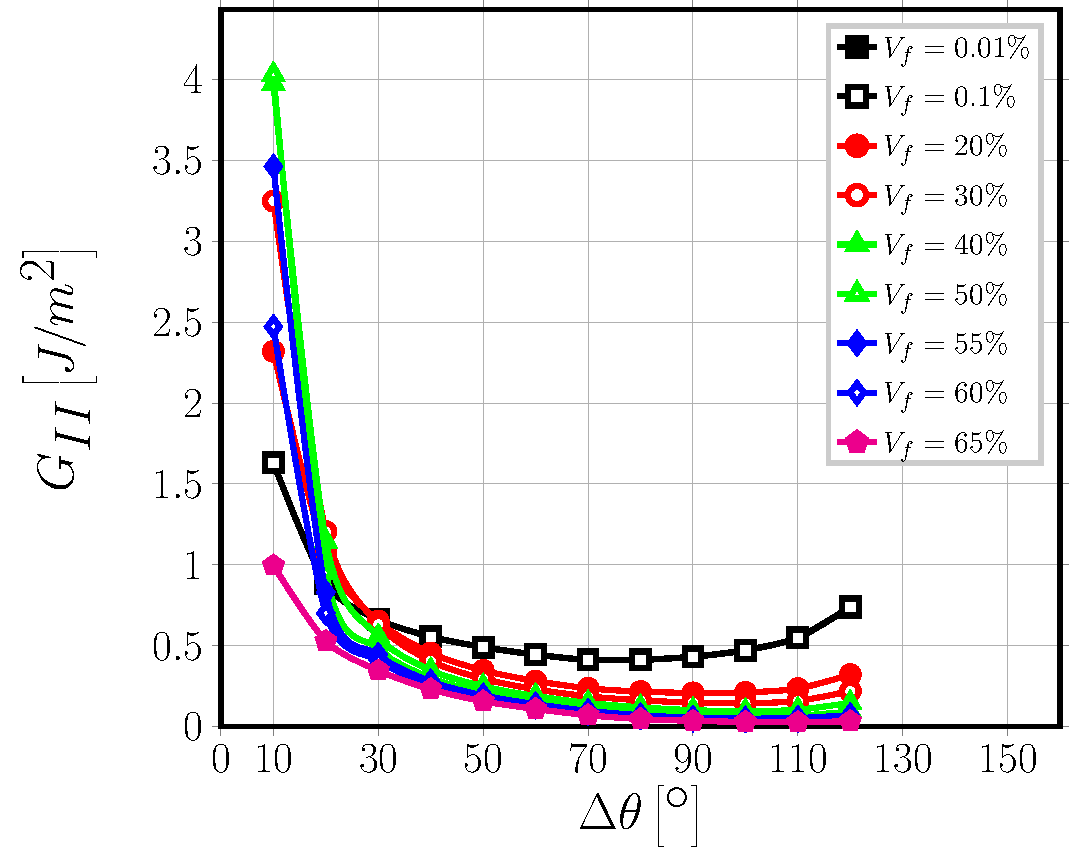
\includegraphics[width=0.9\columnwidth]{GII-free-curvedcrack.pdf}
%\end{figure}
%\end{column}
%\end{columns}
%\end{frame}

\section{Conclusions}

\begin{frame}
\frametitle{Conclusions}
\vspace{-0.5cm}
\centering
\begin{itemize}[label=\ding{212}]
\item $f_{\text{straight crack}}\left(\Delta\theta\right)$: \Checkmark $G_{I}$, \textcolor{red}{\Cross} $G_{II}$\\[10pt]
$f_{\text{inclined crack}}\left(\Delta\theta\right)$: \Checkmark $G_{I}$, \Checkmark $G_{II}$, \textcolor{red}{\Cross} $\nexists\ f_{\text{inclined crack}}\left(\Delta\theta=\frac{\pi}{2}\right)$\\[10pt]
$f_{\text{curved crack}}\left(\Delta\theta\right)$: \Checkmark $G_{I}$, \Checkmark $G_{II}$\\[20pt]
\item scaling breaks for $\Delta\theta\leq20^{\circ}$ $\rightarrow$ microstructure is important for small debonds!
\end{itemize}
\end{frame}

\begin{frame}[plain]
\frametitle{}
\end{frame}

\end{document}
